\documentclass{article}

%%%%%%%%%%%%%%%%%%%%%%%%%%%%%%%%%%%%%%%%%%%%%%%%%%%%%%%%%%%%%%%%%%%%%%
% LATEX DEFINITIONS
%%%%%%%%%%%%%%%%%%%%%%%%%%%%%%%%%%%%%%%%%%%%%%%%%%%%%%%%%%%%%%%%%%%%%%

\usepackage{hyperref}
\usepackage{array}
\usepackage{graphicx}
\usepackage{booktabs}
\usepackage{pifont}
\usepackage{todonotes}
\usepackage{rotating}
\usepackage{color}

\newcommand*\rot{\rotatebox{90}}

\newcommand{\FILE}[1]{\todo[color=green!40]{#1}}

%%%%%%%%%%%%%%%%%%%%%%%%%%%%%%%%%%%%%%%%%%%%%%%%%%%%%%%%%%%%%%%%%%%%%%
% TITLE ABLE OF CONTENTS
%%%%%%%%%%%%%%%%%%%%%%%%%%%%%%%%%%%%%%%%%%%%%%%%%%%%%%%%%%%%%%%%%%%%%%

\newcommand{\TITLE}{The FutureGrid Testbed for Big Data}
\newcommand{\AUTHOR}{Gregor von Laszewsi, Geoffrey C. Fox}
\newcommand{\EMAIL}{laszewski@gmail.com}
\begin{document}

\title{\TITLE}
\author{\AUTHOR}
\date{\EMAIL}


%%%%%%%%%%%%%%%%%%%%%%%%%%%%%%%%%%%%%%%%%%%%%%%%%%%%%%%%%%%%%%%%%%%%%%
% TABLE OF CONTENTS
%%%%%%%%%%%%%%%%%%%%%%%%%%%%%%%%%%%%%%%%%%%%%%%%%%%%%%%%%%%%%%%%%%%%%%

\pagenumbering{roman}

\begin{center}
{\Large\bf \TITLE}\\
{\AUTHOR}\\
{\EMAIL}
\end{center}

\tableofcontents

\newpage

%%%%%%%%%%%%%%%%%%%%%%%%%%%%%%%%%%%%%%%%%%%%%%%%%%%%%%%%%%%%%%%%%%%%%%
% LIST OF TODOS
%%%%%%%%%%%%%%%%%%%%%%%%%%%%%%%%%%%%%%%%%%%%%%%%%%%%%%%%%%%%%%%%%%%%%%

\listoftodos

\newpage

%%%%%%%%%%%%%%%%%%%%%%%%%%%%%%%%%%%%%%%%%%%%%%%%%%%%%%%%%%%%%%%%%%%%%%
% TITLE OF PAPER
%%%%%%%%%%%%%%%%%%%%%%%%%%%%%%%%%%%%%%%%%%%%%%%%%%%%%%%%%%%%%%%%%%%%%%

\pagenumbering{arabic}

\maketitle

%%%%%%%%%%%%%%%%%%%%%%%%%%%%%%%%%%%%%%%%%%%%%%%%%%%%%%%%%%%%%%%%%%%%%%
% ABSTRACT OF PAPER
%%%%%%%%%%%%%%%%%%%%%%%%%%%%%%%%%%%%%%%%%%%%%%%%%%%%%%%%%%%%%%%%%%%%%%


\begin{abstract}

In this chapter we will be introducing you to FutureGrid that provides a testbed to conduct research for Cloud, Grid, and High Performance Computing. Although FutureGrid has only a modest number of compute cores (about 4500 regular cores and 14000 GPU cores) it provides an ideal playground to test out various frameworks that may be useful for users to consider as part of their big data analysis pipelines. 

The chapter is structured as follows. First we will provide the reader with an introduction to Future Grid. We will list a number of projects that use Futuregrid to conduct data analysis and introduce some of them to the reader. We will tell you about which services and Hardware exists. Next we will analyze which services are preinstalled and are available for big data analysis. As services that users may need for their work we point out how such a testbed can be utilized not only while provisioning virtual machines, but also on bare metal. 

We conclude the chapter with our observation cast throught three years of operating FutureGrid and provide an outlook for the next steps.
\end{abstract}

%%%%%%%%%%%%%%%%%%%%%%%%%%%%%%%%%%%%%%%%%%%%%%%%%%%%%%%%%%%%%%%%%%%%%%
% SECTIONS
%%%%%%%%%%%%%%%%%%%%%%%%%%%%%%%%%%%%%%%%%%%%%%%%%%%%%%%%%%%%%%%%%%%%%%

\FILE{introduction.tex}

\section{Introduction}

FutureGrid \cite{las2010gce,las12fg-bookchapter} ``is a project led by Indiana University and funded by the National Science Foundation (NSF) to develop a highperformance grid test bed that will allow scientists to collaboratively develop and test innovative approaches to parallel, grid, and cloud computing. FutureGrid will provide the infrastructure to researchers that allows them to perform their own computational experiments using distributed systems. The goal is to make it easier for scientists to conduct such experiments in a transparent manner.  FutureGrid users will be able to deploy their own hardware and software configurations on a public/private cloud, and run their experiments. They will be able to save their configurations and execute their experiments using the provided tools. The FutureGrid test bed is composed of a highspeed network connecting distributed clusters of high performance computers. FutureGrid employs virtualization technology that will allow the test bed to support a wide range of operating systems.''

The rest of the chapter is structured as follows. 

\todo{Chapter structure}


\section{Overview of FutureGrid}

\FILE{hardware.tex}

\subsection{Hardware Overview}

According to the manual, FutureGrid is build out of a number of clusters of different type and size that are interconected with up to a 10GB Ethernet among its sites. The sites include Indiana University, University of Chicago, San Diego Supercomputing Center, Texas Advanced Computing Center, and University of Florida.

\subsubsection{Overview of the Clusters}\label{S:hw-cluster} 

\begin{table}[htb]

\caption{FutureGrid Compute Resources}\label{T:hw}

\begin{center}
\begin{tabular}{rrrrrrrrr}
Name    & System Type                &  \rot{Nodes} &  \rot{CPUS}   & \rot{Cores}   & \rot{TFLOPS}  & \rot{RAM (GB)}        & \rot{Storage (TB)}    & Site \\
\hline
india   & IBM iDataplex              & 128          & 256     & 1024    & 11      & 3072            & 335             & IU \\
hotel   & IBM iDataplex              & 84           & 168     & 672     & 7       & 2016            & 120             & UC \\
sierra  & IBM iDataplex              & 84           & 168     & 672     & 7       & 2688            & 96              & SDSC \\
foxtrot & IBM iDataplex              & 32           & 64      & 256     & 3       & 768             & 0               & UF \\
alamo   & Dell Poweredge             & 96           & 192     & 768     & 8       & 1152            & 30              & TACC \\
xray    & Cray XT5m                  & 1            & 166     & 664     & 6       & 1328            & 5.4             & IU \\
bravo   & HP Proliant                & 16           & 32      & 128     & 1.7     & 3072            & 128             & IU \\
delta   & \shortstack{SuperMicro\\ GPU Cluster}     & 16           & 32      & 192     &         & 1333            & 144             & IU \\
lima    & Aeon Eclipse64             & 8            & 16      & 128     & 1.3     & 512             & 3.8             & SDSC \\
echo    & \shortstack{SuperMicro \\ScaleMP Cluster} & 16           & 32      & 192     & 2       & 6144            & 192             & IU \\
\end{tabular}
\end{center}
\end{table}


\begin{sidewaystable}

\caption{FutureGrid cluster details.}\label{F:cluster-details}
~\\
\begin{footnotesize}
\begin{tabular}{|p{2cm}||p{4cm}p{1.5cm}p{1.5cm}p{1.5cm}p{1.5cm}p{1.5cm}p{1.5cm}p{1.5cm}p{1cm}|}
\hline
 \bf Name                                & \bf Echo & \bf Alamo & \bf Bravo & \bf Delta & \bf Foxtrot & \bf Hotel & \bf India & \bf Sierra & \bf Xray \\
\hline
\hline
 Organization                        & IU & TACC & IU & IU & UF & UC & IU & SDSC & IU \\
\hline
 Machine Type                        & Cluster SclaeMP & Cluster & Cluster & Cluster & Cluster & Cluster & Cluster & Cluster & Cluster \\
\hline
 System Type                         &SuperMicro& Dell PowerEdge M610 Blade & HP Proliant && IBM iDataPlex dx 360 M2 & IBM iDataPlex dx 360 M2 & IBM iDataPlex dx 360 M2 & IBM iDataPlex dx 340 & Cray XT5m \\
\hline
 CPU Type                            & Xeon E5-2640 &  Xeon X5550 &  Xeon E5620 &  Xeon 5660 &  Xeon X5520 &  Xeon X5550 &  Xeon X5550 &  Xeon L5420 & Opteron 2378 \\
\hline
 CPU Speed                           &2.50GHz& 2.66GHz & 2.40GHz & 2.80 GHz & 2.26GHz & 2.66GHz & 2.66GHz & 2.5GHz & 2.4GHz \\
\hline
 CPUs                                &&192&32&32&64&168&256&168&168 \\
\hline
 Servers                             &12&96&16&16&32&84&128&84&1 \\
\hline
 RAM                                 && 12GB DDR3 1333Mhz & 192GB DDR3 1333Mhz & 192GB DDR3 1333 Mhz & 24GB DDR3 1333Mhz & 24GB DDR3 1333Mhz & 24GB DDR3 1333Mhz & 32GB DDR2-667 & 8GB DDR2-800 \\
\hline
 Total RAM                           &&1152GB&3072GB&3072GB&768GB&2016GB&3072GB&2688GB&1344GB \\
\hline
 Number of cores                     &144&768&128&&256&672&1024&672&672 \\
\hline
 Tflops                              &&8&1.7&&3&7&11&7&6 \\
\hline
 Disk Size (TB)                      &2.8&48&&15&20&120&335&72&335 \\
\hline
 Hard Drives                         && 500GB 7.2K RPM SAS & 6x2TB 7.2K RPM SATA & 92GB 7.2K RPM SAS2 & 500GB 7200 RPM SATA & 1 TB 7200 RPM SATA & 3000GB 7200 RPM SATA & 160GB 7200 RPM SATA Drive & 6TB Lustre \\
\hline
 Shared Storage                      && NFS & NFS &NFS& NFS & GPFS & NFS & ZFS 82.2TB & NFS \\
\hline
 Interconnect                        && Mellanox 4x QDR IB & Mellanox 4x DDR IB &&& Mellanox 4x DDR IB & Mellanox 4x DDR IB & Mellanox 4x DDR IB & Cray SeaStar \\
\hline
\end{tabular}
~\\
IB = InfiniBand, Xenon = INtel Xenon, Opteron = AMD Opteron 

\end{footnotesize}

\end{sidewaystable}



\subsubsection{Overview of Networking}

The significant number of distinct systems within FutureGrid provide a
heterogeneous distributed architecture and are connected by
high-bandwidth network links supporting distributed system research
\cite{las12fg-bookchapter}. FutureGrids network used to have a
dedicated network between sites \cite{las12fg-bookchapter}. However,
the network infrastructure has recently changed due to changes as part
of its major network operator the National Lambda Rail.  Due to these
changes the operation of the network between the sites conducted by
the national lambda rail has switched opertaion to XSEDE and are no
longer exclusive. This is no major handicap for the projects conducted
on FutureGrid based on our project portfolio.  The current high level
network diagram is depicted in Figure~\ref{F:network}.

The core resources to FutureGrid at SDSC, IU, TACC, and UF are now all
connected via the XSEDE network and integrated via the FG core router
in Chicago. WIthin The IU network additional clusters are integrated
and are described in more detail in Section~\ref{S:hw-cluster}. 

A Spirent H10 XGEM Network Impairment emulator
\cite{www-network-impairment} can be colocated with resources at
Indiana University, to enable experiments to include network latency,
jitter, loss, and errors to network traffic.

In addition we have added several shaded components that are related
to a spcial software service called cloudmesh that we explain in more
detail in Section~\ref{S:cloudmesh}.


\begin{figure}[htb]
  \centering
    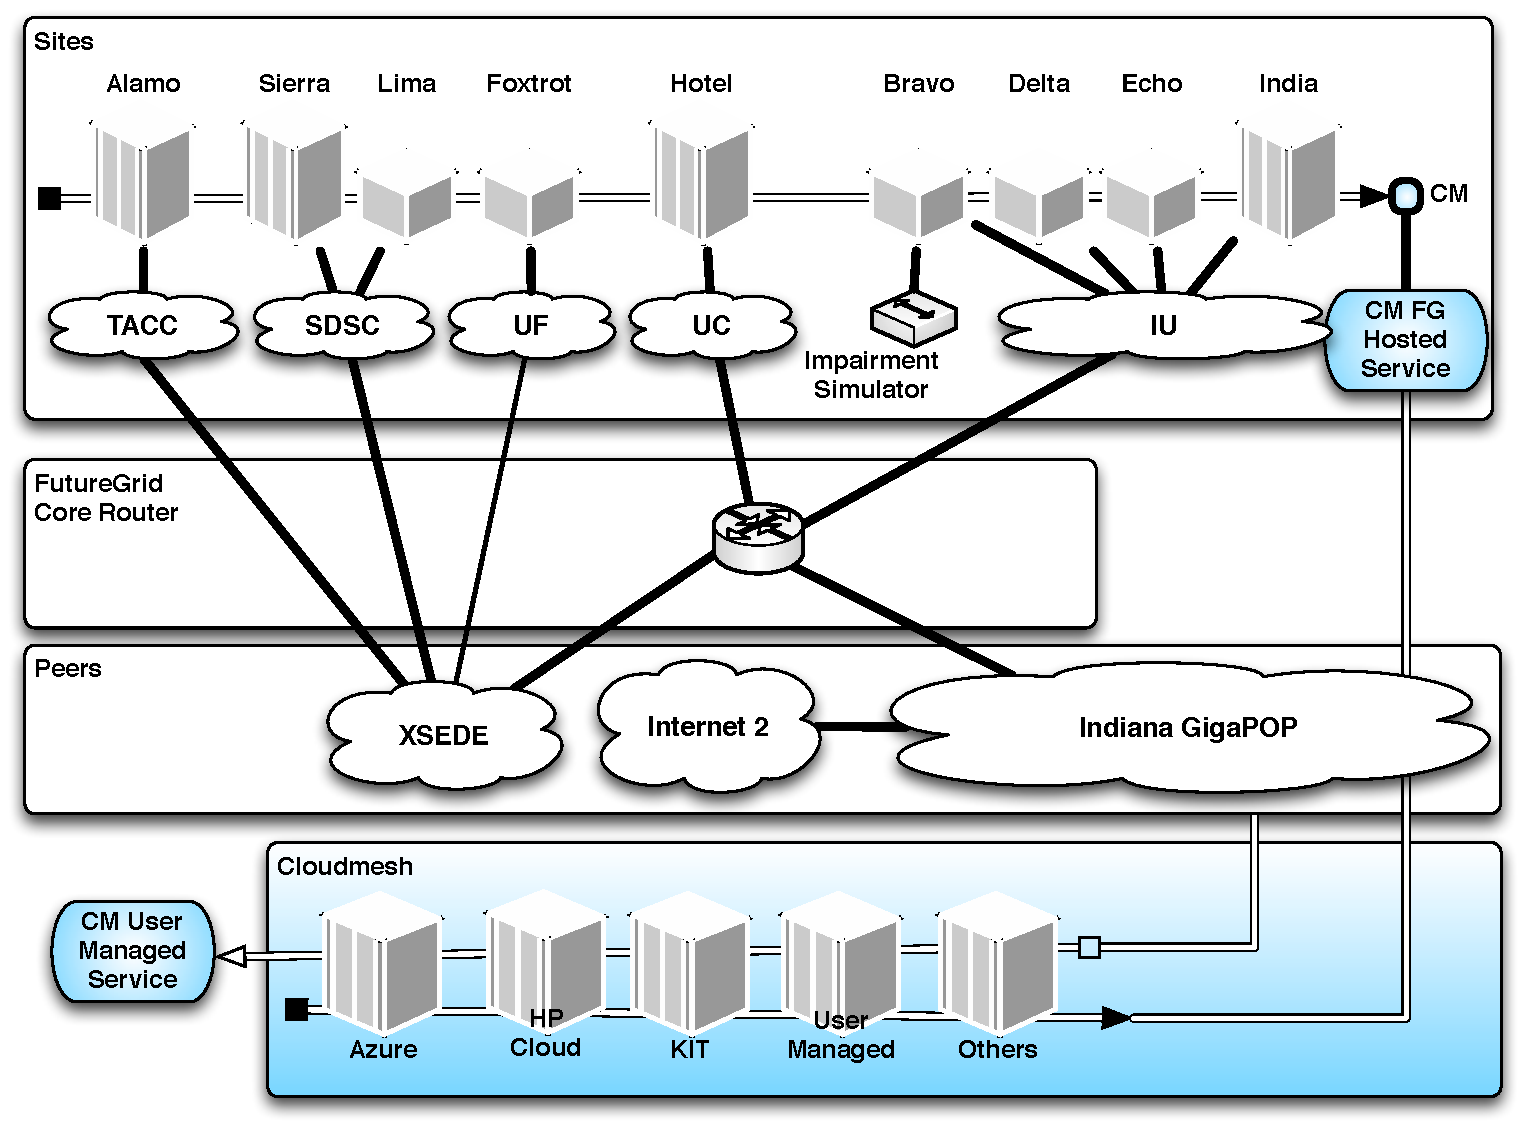
\includegraphics[width=1.0\textwidth]{images/fg-network-2014-cm.pdf}
  \caption{High level network diagram and conceptual integration of cloudmesh resources.}
\label{F:network}
\end{figure}

\subsubsection{Overview of Storage}

FutureGrid has only a very limited amount of storage space and users
are requested to remove their storage space after use. GutureGrid does
not provide capacity for long term storage or long term
experiments. Users with special needs may be acomodated by special
storage setups. The list of storage services is shown in Table \ref{T:storage}.

\begin{table}[htb]
\caption{Storage Resources of FutureGrid.}
\label{T:storage} 

\centering{}%
\begin{tabular}{lrll}
\textbf{System Type } & \textbf{Capacity(TB) } & \textbf{File System } & \textbf{Site }\tabularnewline
\hline 
Xanadu 360  & 180  & NFS  & IU \tabularnewline
DDN 6620  & 120  & GPFS  & UC \tabularnewline
Sunfire x4170  & 96  & ZFS  & SDSC \tabularnewline
Dell MD3000  & 30  & NFS  & TACC \tabularnewline
IBM dx360 M3  & 24  & NFS  & UF \tabularnewline
\end{tabular}
\end{table}



\todo{services.tex}

\subsection{Service Overview}

According to the manual FutureGrid provides a number of different
services. These services include:

\begin{enumerate}
\item OpenStack which includes a collection of open source components to deliver public and private clouds. These components currently include OpenStack Compute) OpenStack Object Storage, and OpenStack Image Service. OpenStack has received considerable momentum due to its openness and the support of companies. 

\item Nimbus which is an opensource service package that allows users to run virtual machines on FutureGrid hardware. Just as in Openstack users can upload their own virtual machine images or customize existing once. Nimbusnext to Eucalyptus is one of the earlier frameworks that make managing virtual machines easier.

\item Eucalyptus is an opensource software platform that implements IaaS-style cloud computing. Eucalyptus provides an Amazon Web Services (AWS) compliant EC2-based web service interface for interacting with the Cloud service.  Eucalyptus has been previously the dominant alternative to AWS  in academia. However, based on usage patterns in FutureGrid we believe it is replaced by OpenStack.

\item High Performance Computing can be defined as the application of supercomputing techniques to solve computational problems that are too large for standard computers or would take too much time. This is one of the more important features that the scientific community needs to achieve their projects. Naturally using HPC resouces and services is also useful in the area of Big Data. Sometimes big data needs big machines. Thus, using HPC may be an ovious choice.

\item Map Reduce …. TBD …

\end{enumerate}

Storage on FutureGrid has moderate size storage capability that will satisfy the users demand to compare and test someof the previously outlined services.

Information Services gather the information of the different elements that make up FutureGrid to provide accurate and complete knowledge of the computational environment. This information is presented using different web portals.

\begin{figure}[p]
  \centering
    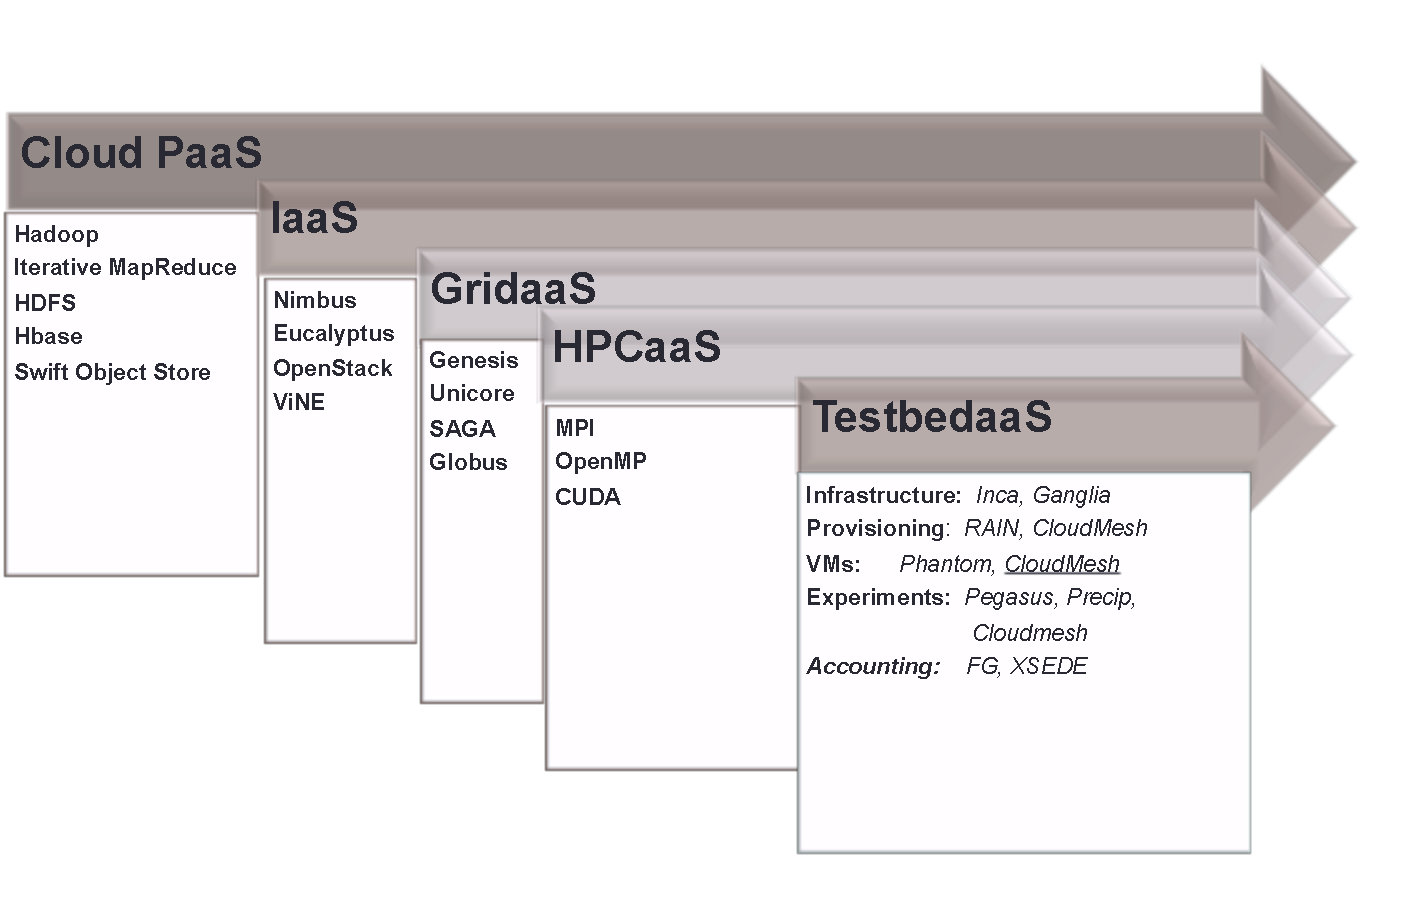
\includegraphics[width=0.9\textwidth]{images/user-services.pdf}
  \caption{FutureGrid High Level User Services.}
  ~\\
  \centering
  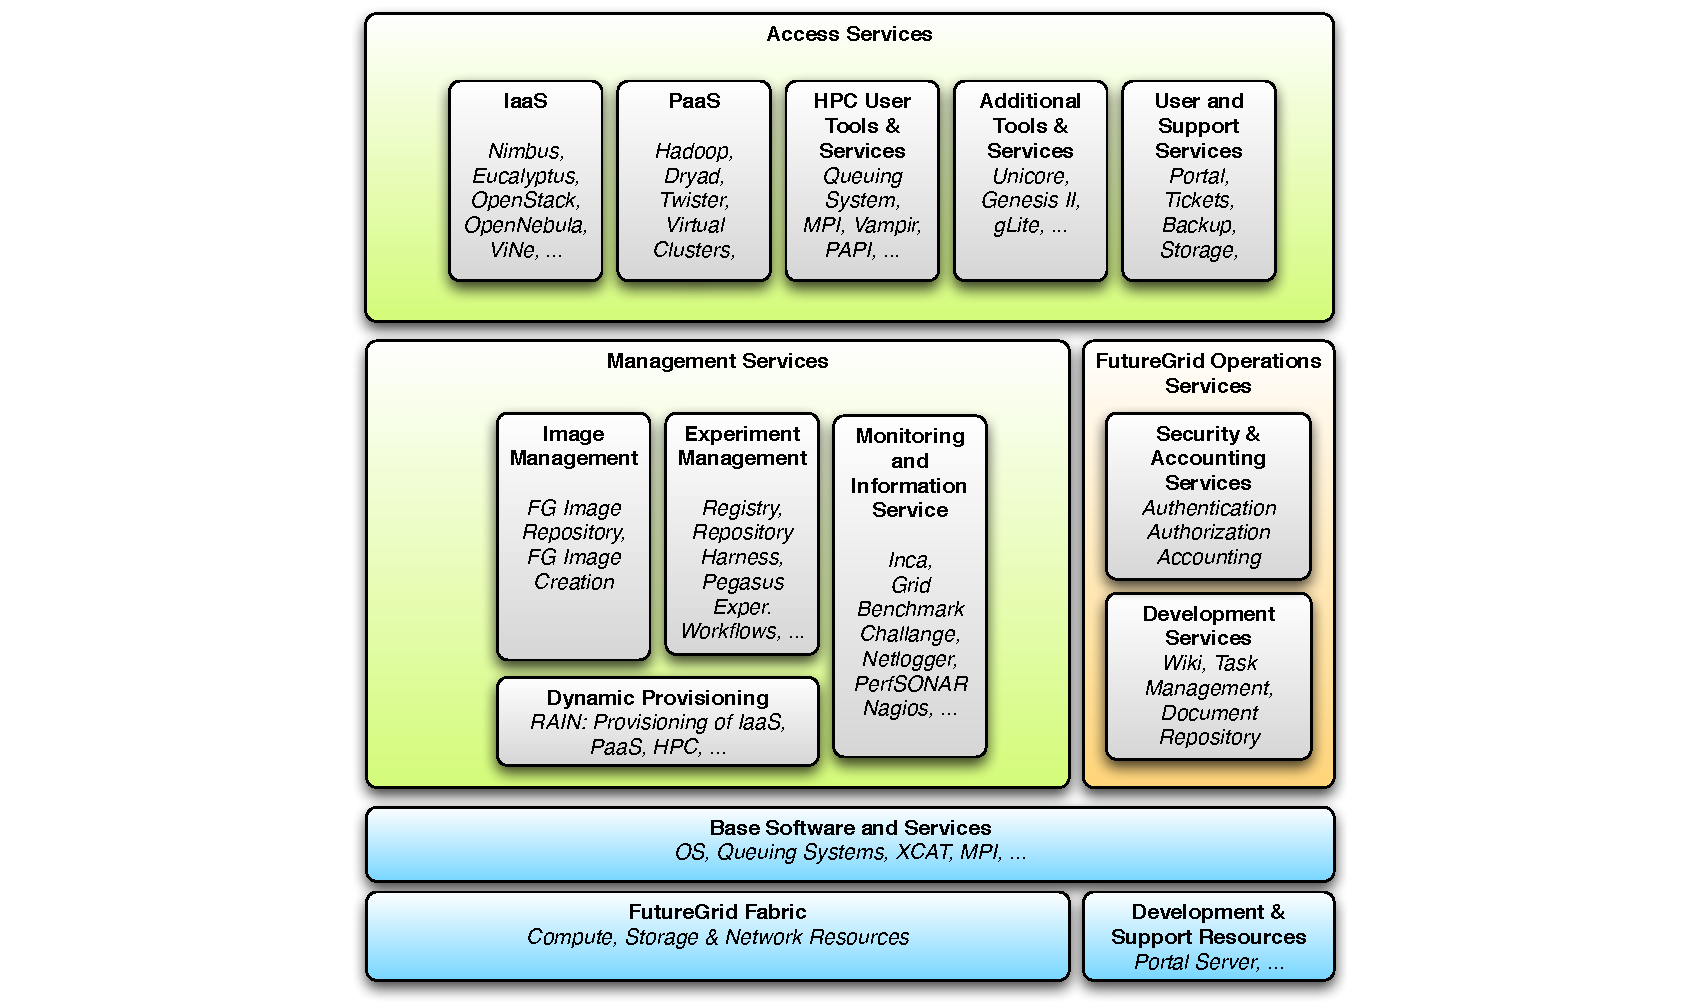
\includegraphics[width=0.9\textwidth]{images/architecture.pdf}
  \caption{Architecture.}
\end{figure}


\FILE{usage.tex}

\section{FutureGrid Usage}

When offering services such as FutureGrid to the community, we have to
analyse and predict which services may be useful for the users. We
have therefore established a number of activities that monitor
external and interanl data. Externally, we look for example at
information provided by Gartners technology hype curve \cite{?} or
Google trend information as shown in Figure \ref{F:google-trend}. From
Google Trend data we observe that the populariity of Grid computing
has been very low  in the recent years and much attention has shifted
to cloud computing. Therefore we removed this information from the
figure and focuss exemplary on cloud related terms such as {\em Cloud
  Computing}, {\em Big Data}, {\em OpenStack} {\em VMWare}.
From this information we see that all but VMWare are rising, with
Cloud Computing dominating the google trends in comparision to the
others. This trend is important as it shows a shift in the cloud
computing community buzz away from a traditional commecial market
leader in virtualization technology. We believe that is correlated
with a large number of vendors offering alternative prducts and
services while at the same time the novelty from VMWare is reduced.

\begin{figure}[htb]
 \centering
    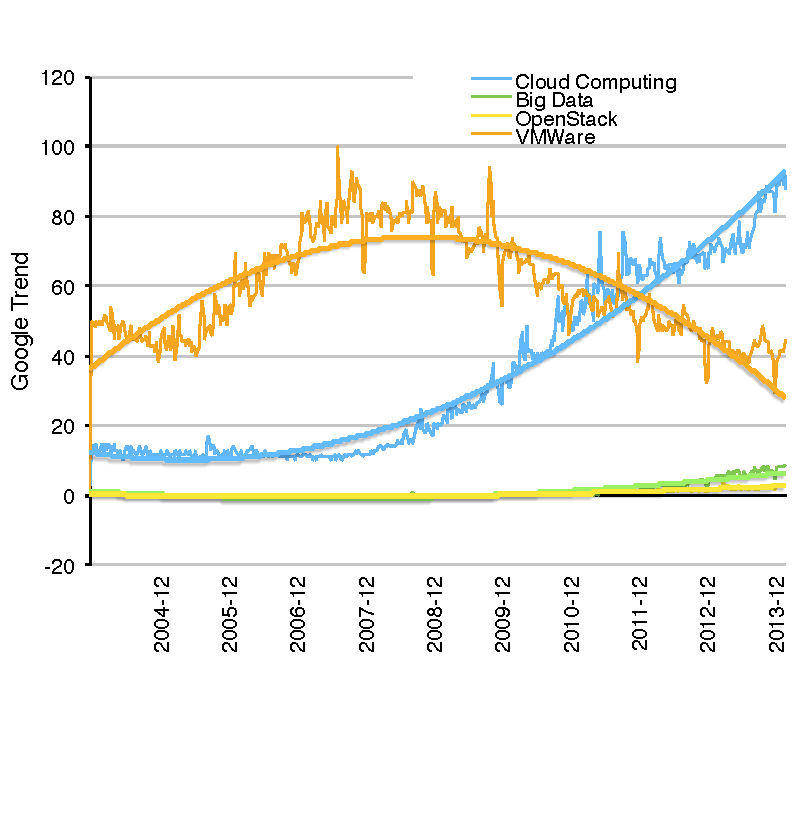
\includegraphics[width=.75\textwidth]{images/google-trend.pdf}
  \caption{Google Trends.}\label{F:google-trend}
\end{figure}

To give an informal overview of the more than 300 projects conducted
on FutureGrid we have taken their titles and display them in a word
cloud (see Figure \ref{F:wordcloud}. Additionally, we have taken
keywords that are provided by the project leades and also displayed
the in a word cloud (see Figure \ref{F:keycloud}. Although the
imagesdoe not give quantitative perspective about the project it helps
to identify some rough idea about the activities that are ongoing in FutureGrid.
As expected the terms cloud computing an and terms such as mapreduce,
Openstack, Nimbus, and Eucalyptus appear quite frequently. It is hence
worthwhile to analyse this data in a more quantitative form.

\begin{figure}[htb]
\begin{minipage}[t]{0.5\textwidth}
  \centering
    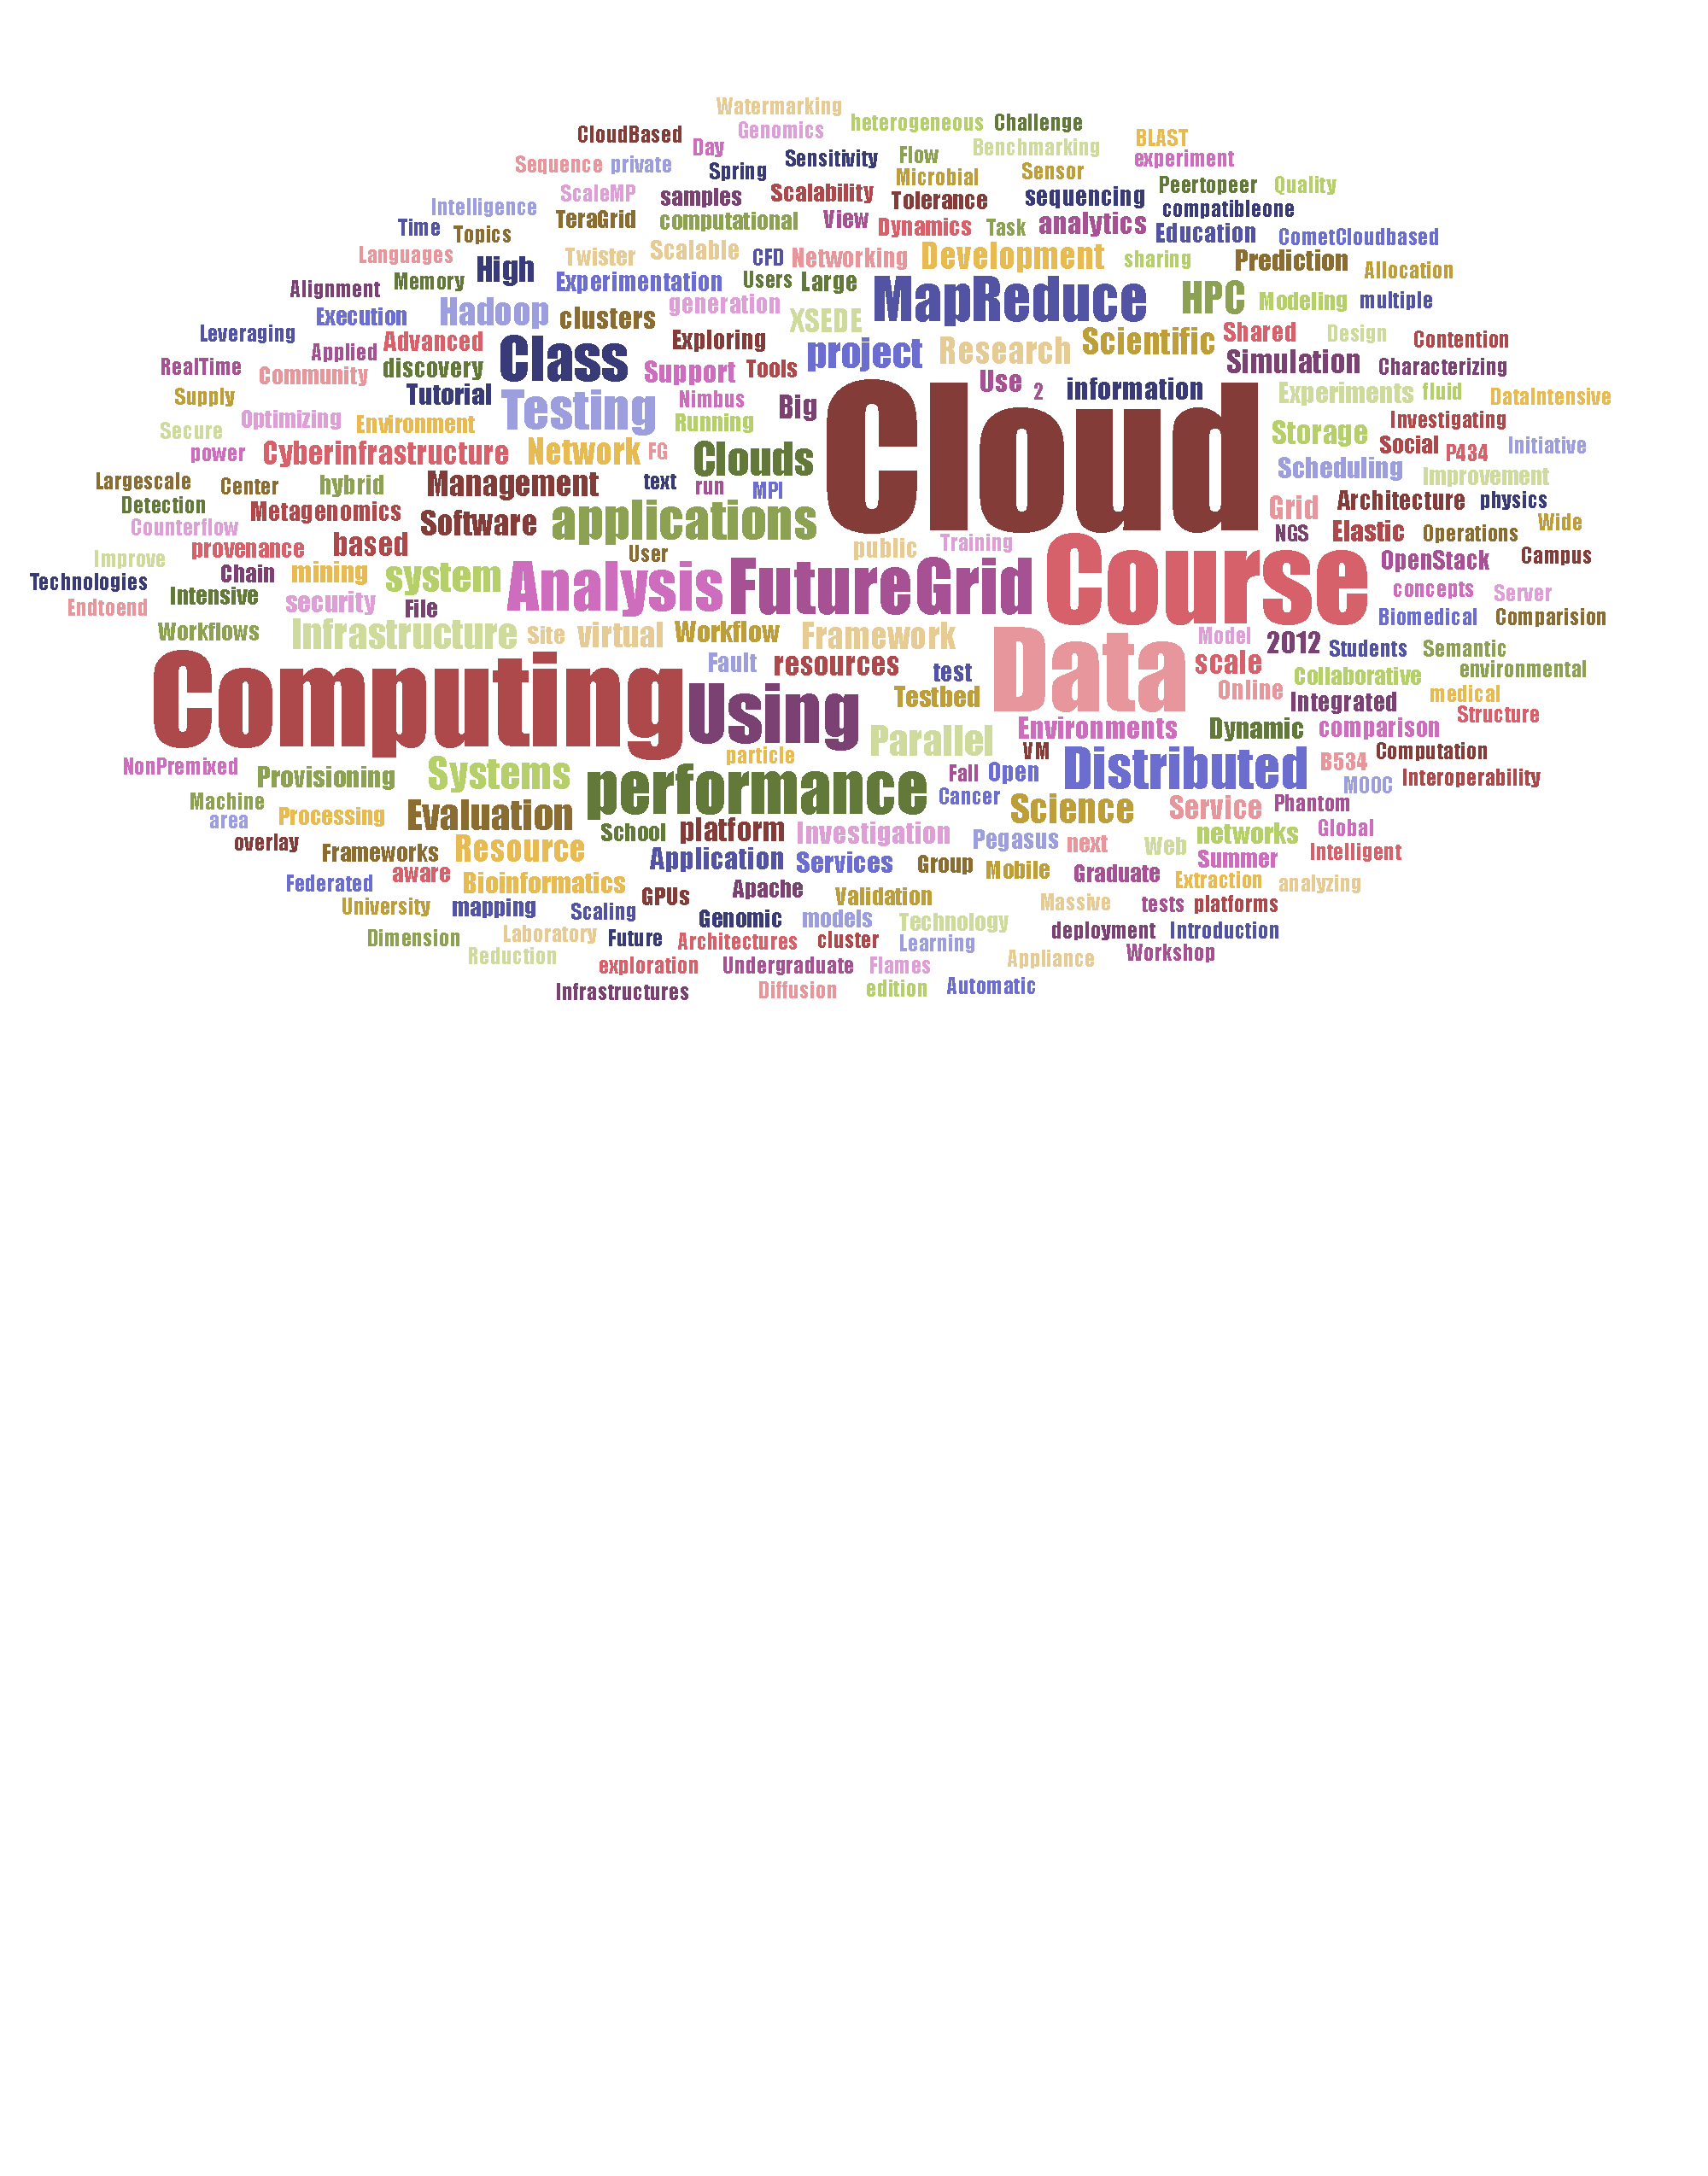
\includegraphics[width=1.0\textwidth]{images/fg-title-wordcloud.pdf}
  \caption{Project title word cloud.}\label{F:wordcloud}
\end{minipage}
\begin{minipage}[t]{0.5\textwidth}
  \centering
    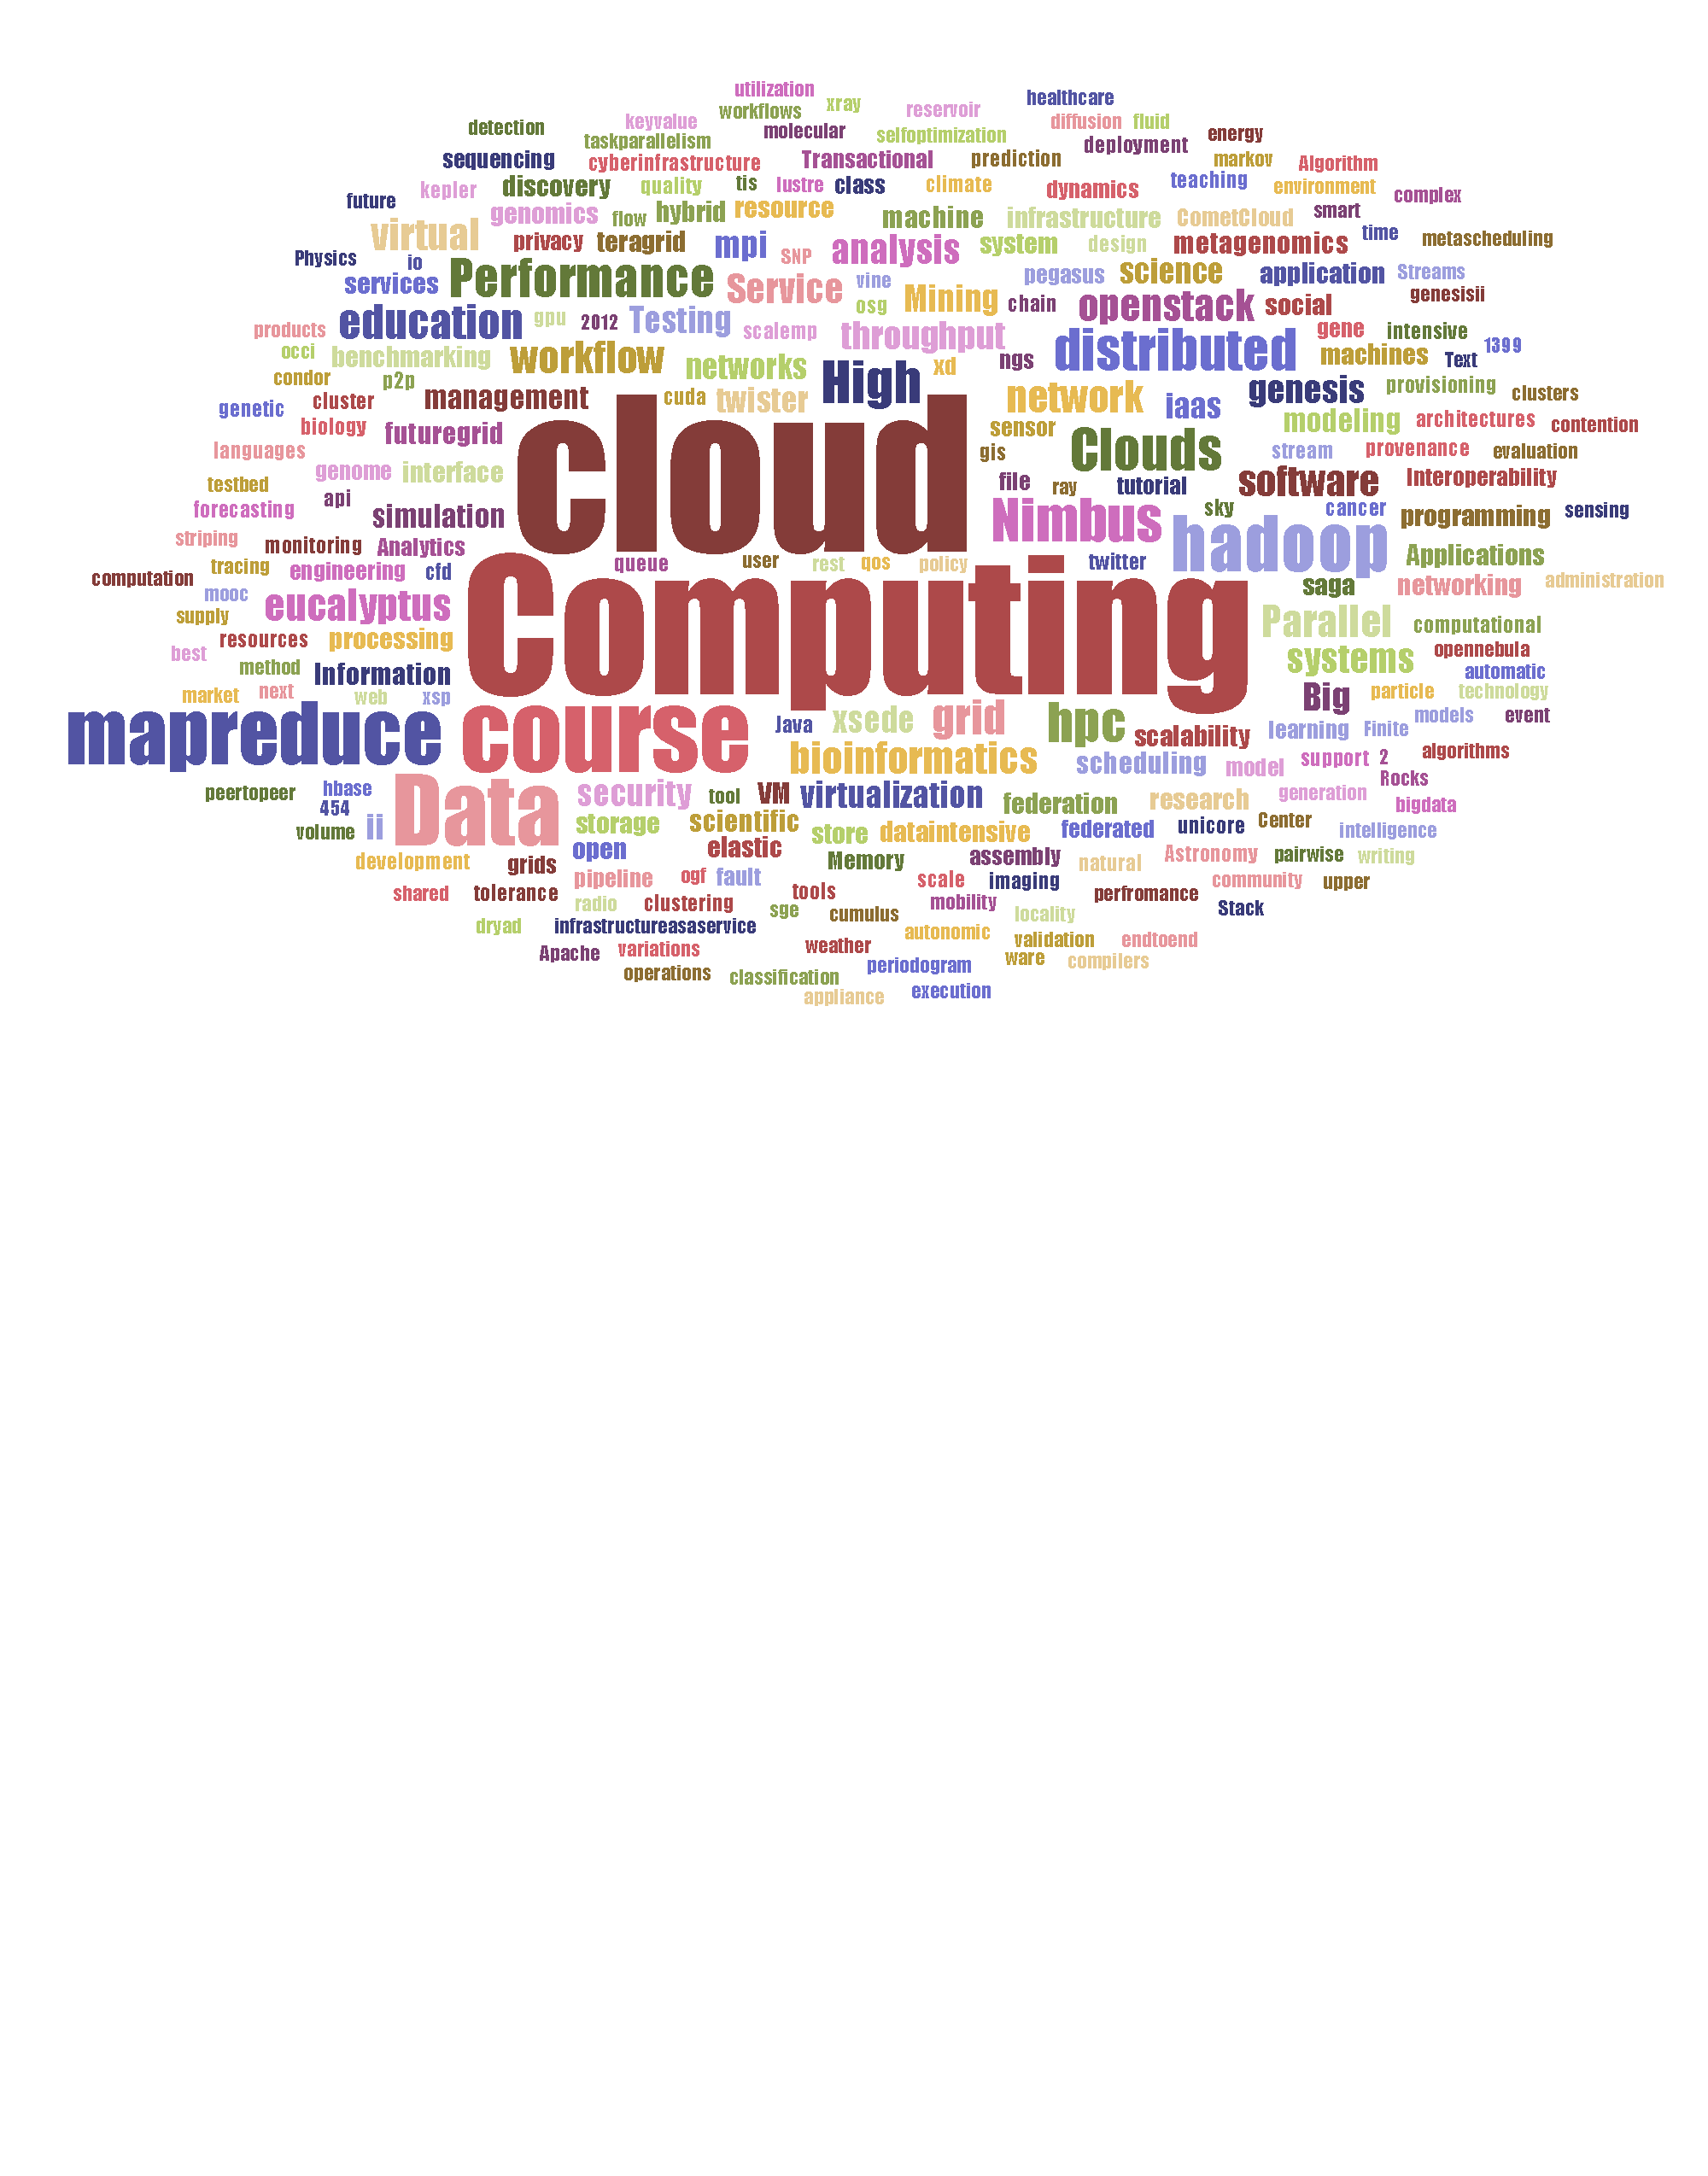
\includegraphics[width=1.0\textwidth]{images/fg-keyword-wordcloud.pdf}
  \caption{Project keyword word cloud.}\label{F:keycloud}
\end{minipage}
\end{figure}


As part of our project management in FutureGird we have designed a
simple project application procedure that includes prior to a project
granted access gathering information about which technologies are
anticipated to be used within the project. The list is fairly
extensive and includes Grid, HPC, and Cloud computing systems,
services, and software. However, for this paper we will focus
primerally on technologies that are dominantly requested and depicted
in Figure~\ref{F:request-tech}. Clearly we can identify the trend,
that shows the increased popularity of OpenStack within the services
offered on FutureGrid. Nimbus and Eucalyptus are on a significant
downwards trend. ObenNebula was also at one point more reqested that
either Nimbus or Eucalyptus, but do to limited manpower an official
version of OpenNebula was not made available. As we have not offered
it and pointed it out on our Web page, requests for OpenNebula have vanished.
However internally have used OpenNebula for projects such as our cloudmesh rain
framework. All other sixteen technologies are relatively equally
distributed over the monitoring period. The lesson that we took form
this is that FutureGrid has put more emphasize in offereing OpenStack Services.

\begin{figure}[htb]
  \centering
    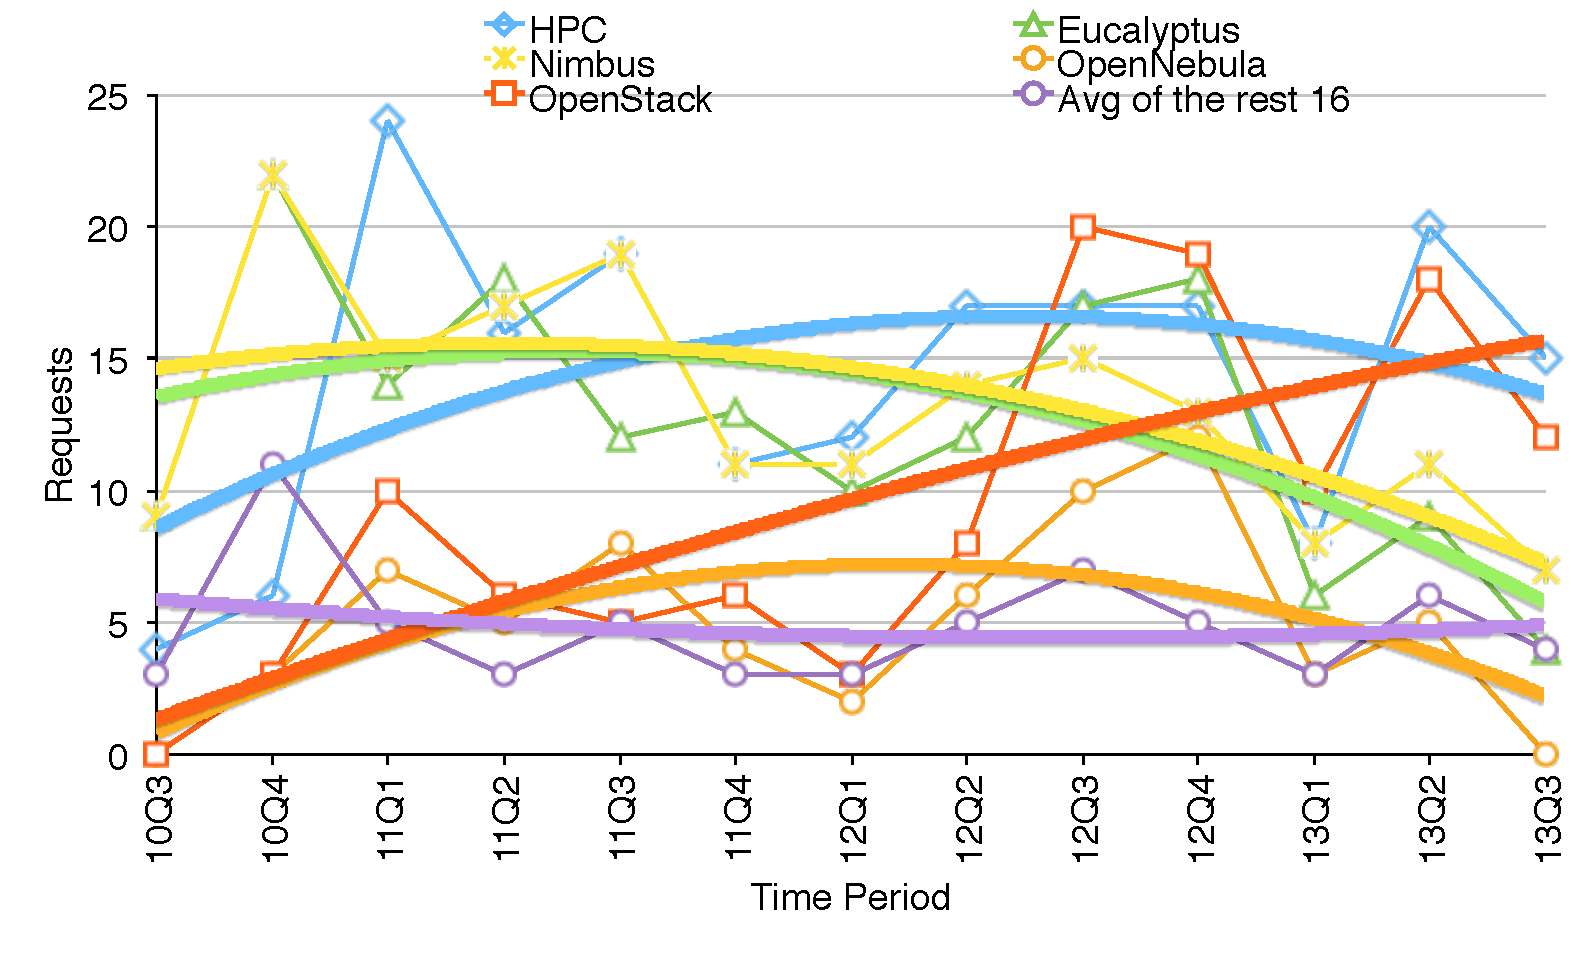
\includegraphics[width=1.0\textwidth]{images/trend-a.pdf}
  \caption{Requested technologies by project}\label{F:request-tech}
\end{figure}

From the overall project information we have also analysed the
frequency of the number of project members within the project and show
it in Figure~\ref{F:project-members}. Here we depict on the abscissa
classes of projects with varying members.  Assume we look at the
abscissa value of 10, This means that thease are all projects that
have project members between 10 and its previous category in this case
5. Hence, it will be all projects greater  5 and smaller or equal
10. With this calsssification  we see that the dominant unique number of
members within all projects is either one, two or thre members. Than
we have another class between 4 and 10 members, and the rest with more
than ten members. One of the projects had overall 186 registered
members, for an education class as part of a summer school. Looking at
the distribution of the members and associating them with reserach and
education projects, we find all projects with larger numbers of
projects to be education projects.


\begin{figure}[htb]
 \centering
    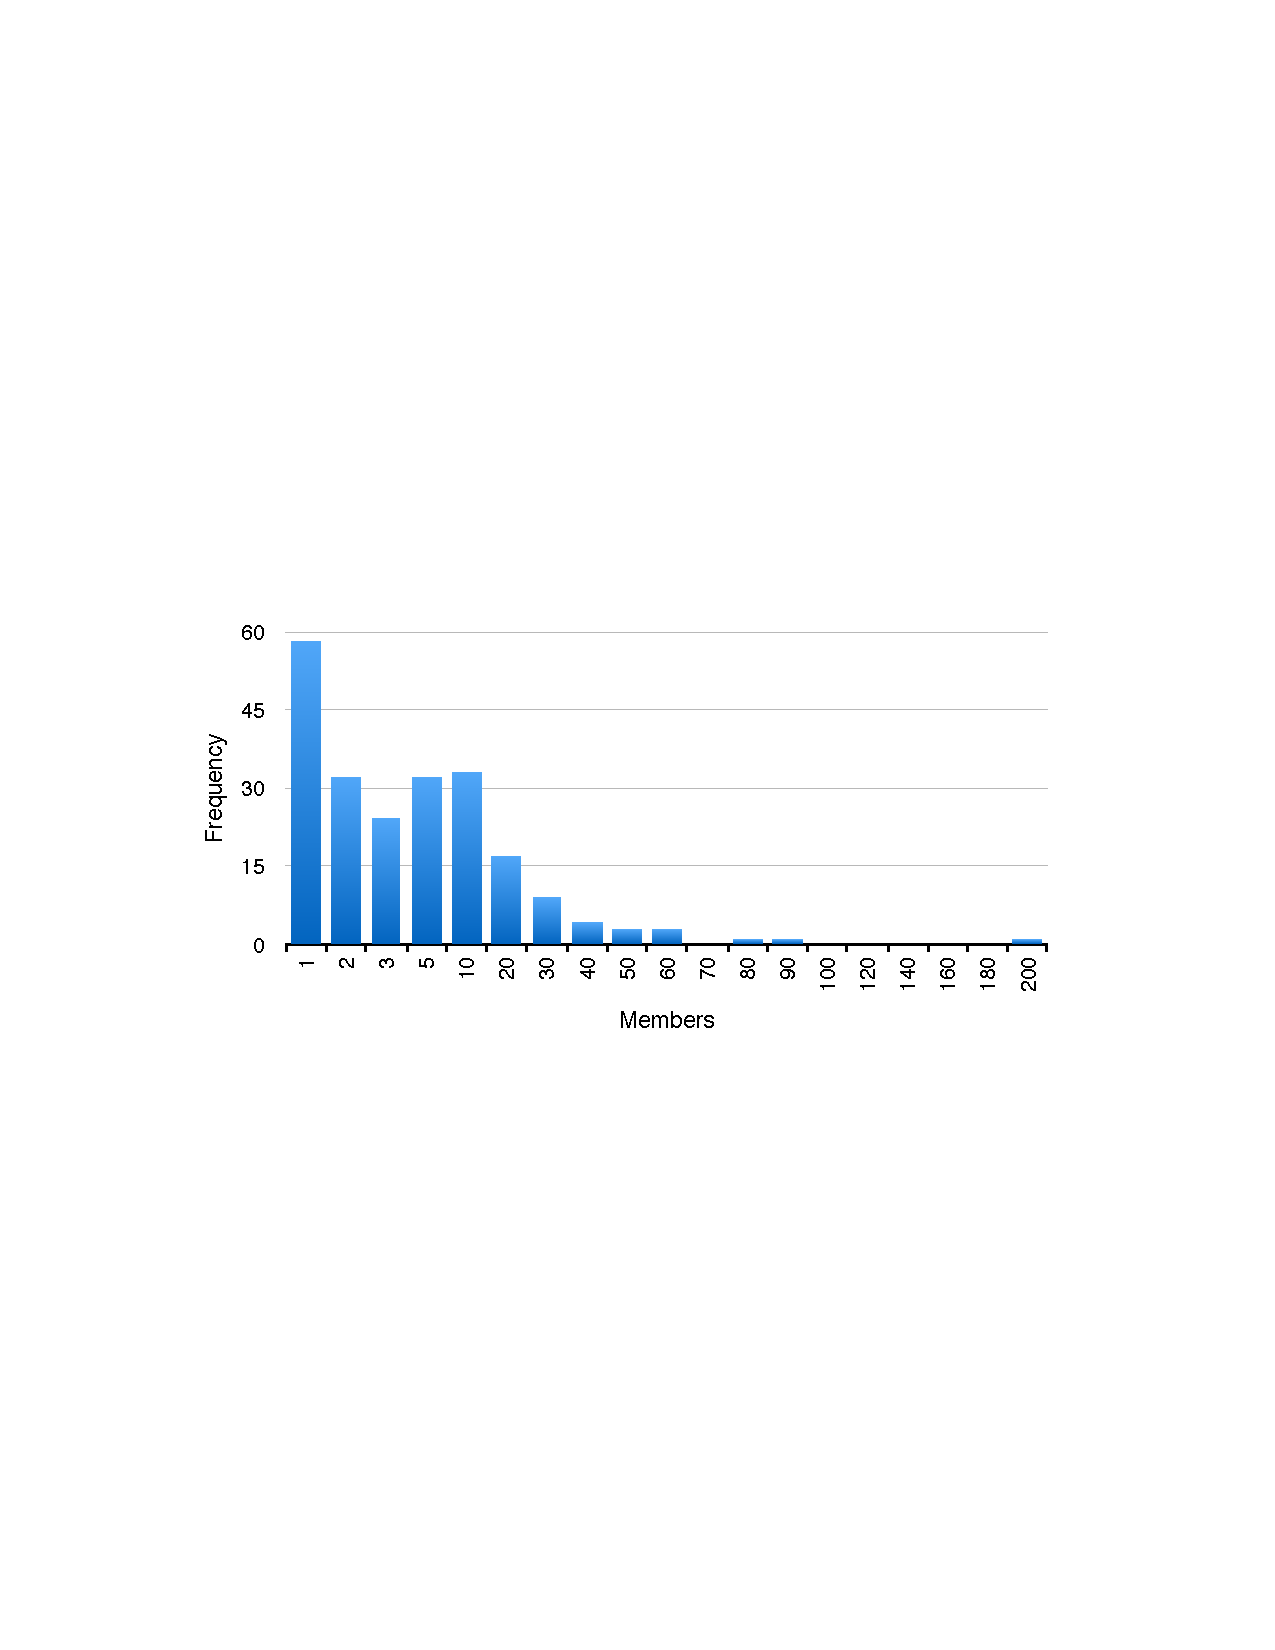
\includegraphics[width=1.0\textwidth]{images/project-frequency.pdf}
  \caption{Project Frequency.}\label{F:project-members}
\end{figure}

%Figure~\ref{F:bigdata-freq} shows the frequency distribution of technologies such as
%map/reduce, hadoop, and twister by year. In the chart we simply called
%the agglomoration of these technologies big data.  As we see relative
%to all projects requested within one year we identified a rising trend.

%\begin{figure}[htb]
%  \centering
%    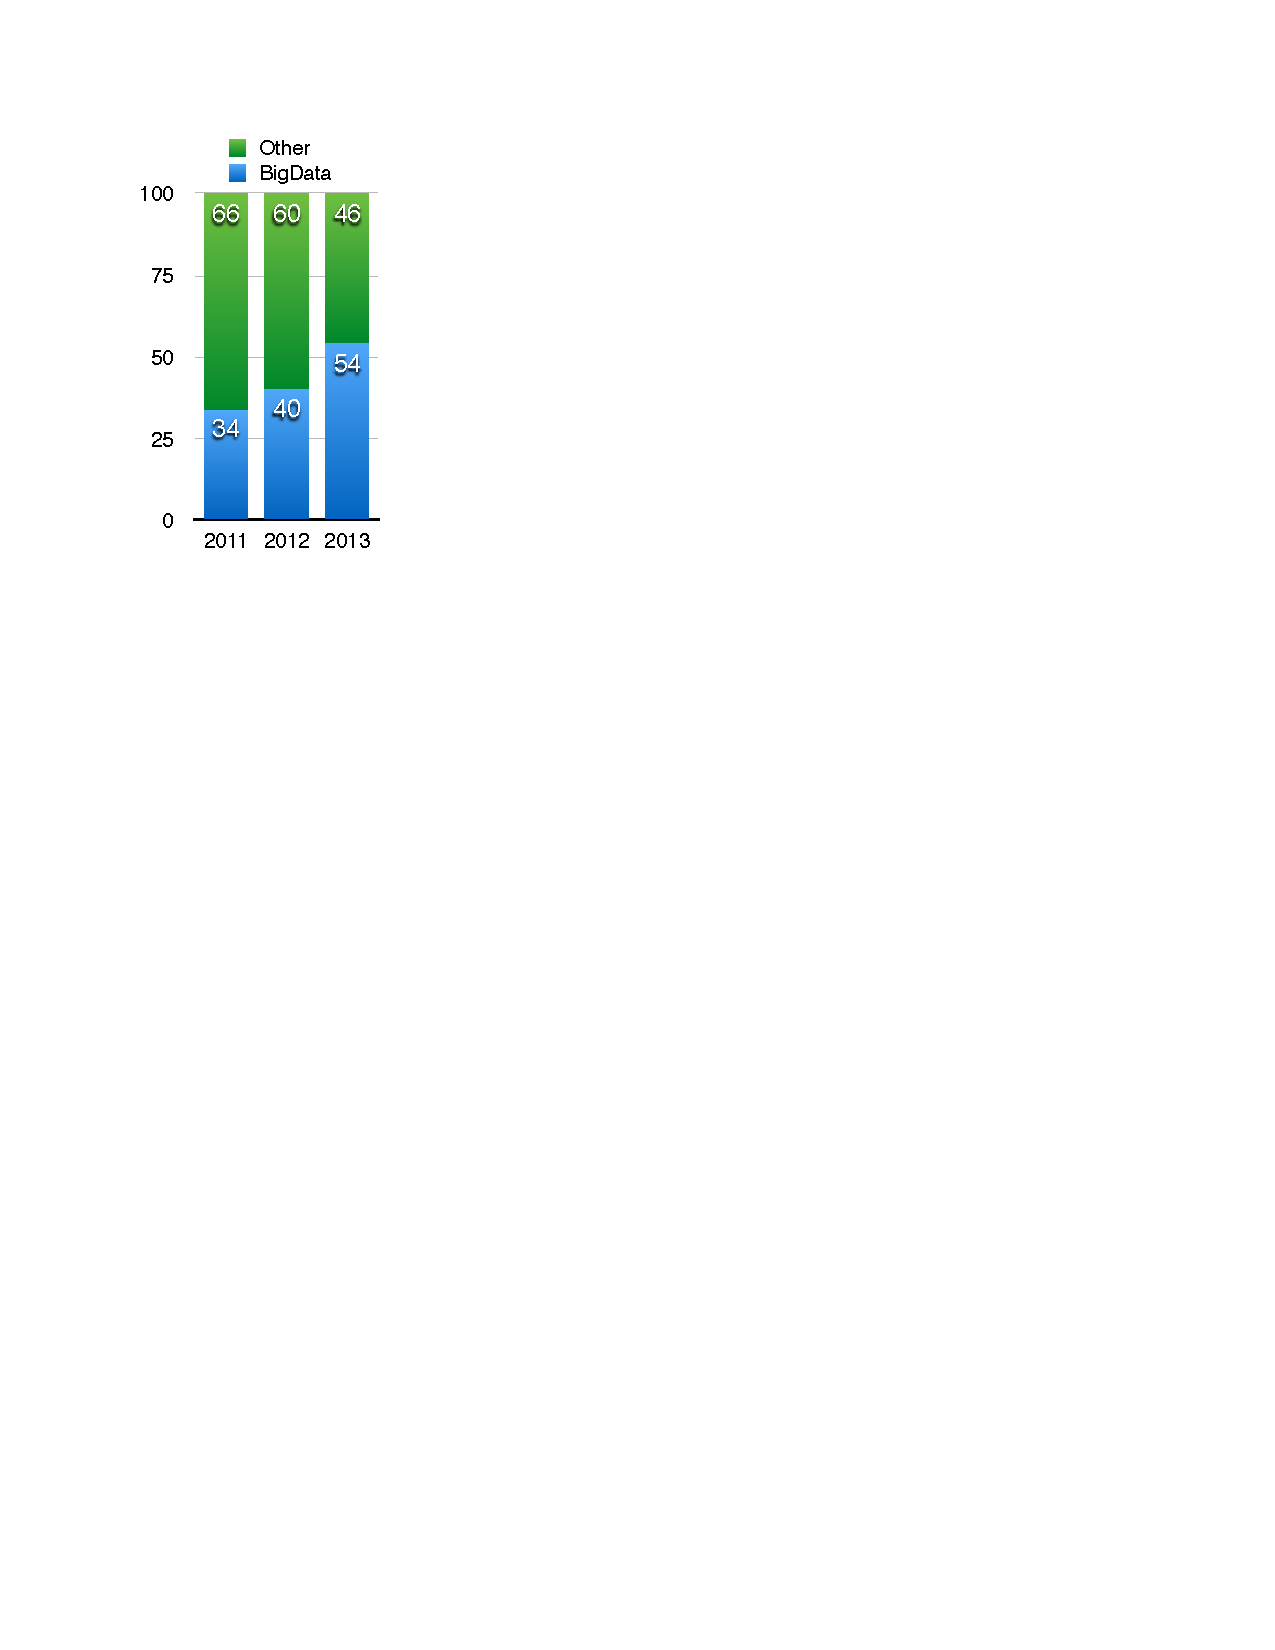
\includegraphics[width=0.2\textwidth]{images/bigdata-freq.pdf}
%  \caption{Big Data Project frequency.}\label{F:bigdata-freq}
%\end{figure}

Next we have taken from all projects in the categories as depicted in
\ref{F:freq-dis}. In contrast to XSEDE which provides a production HPC
system to the scientific community, the usage of FutureGrid is
dominated with 50\% by computer science related projects\footnote{is
  this for all projects or just within hadoop? This is not cear from
  the data I received.} Education is the next highest with 19\%.

\begin{figure}[htb]
  \centering
    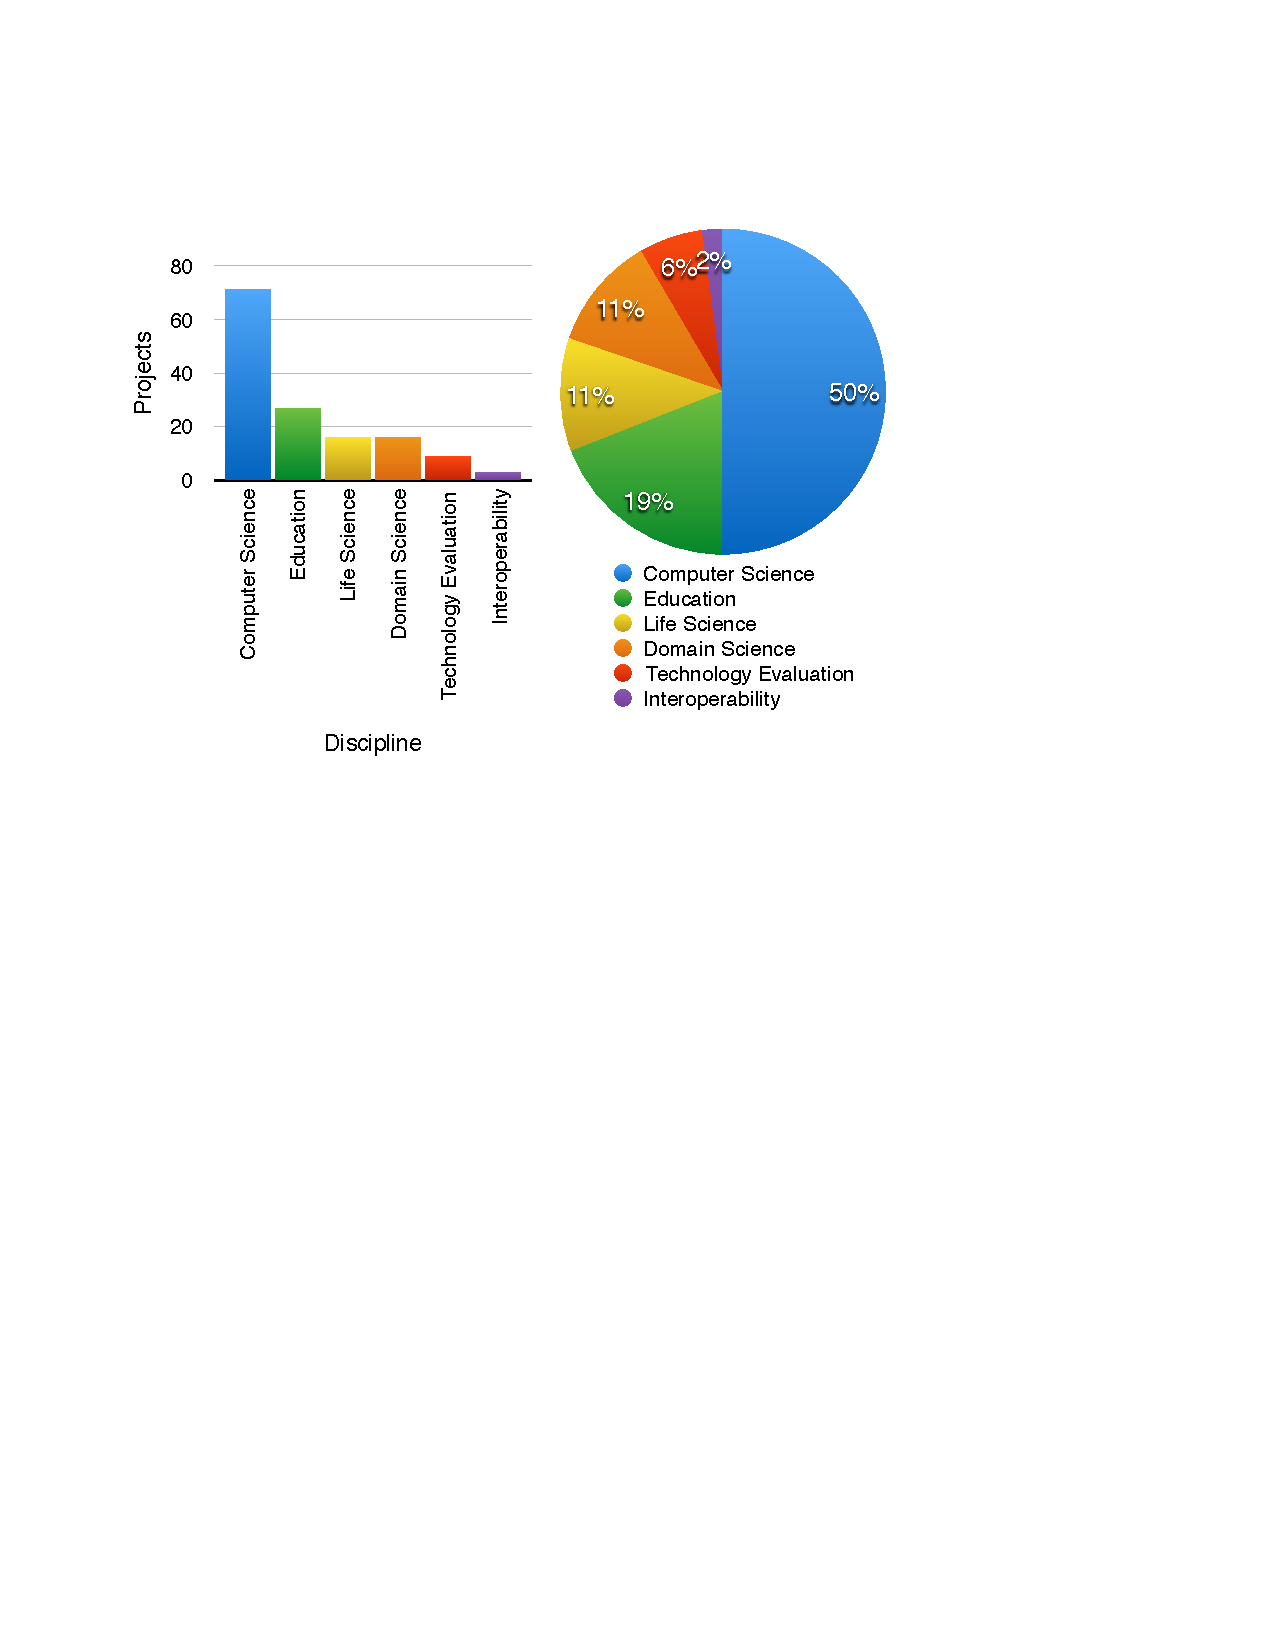
\includegraphics[width=1.0\textwidth]{images/project-disciplines.pdf}
  \caption{project disciplines.}
  \label{F:freq-dis}
\end{figure}

If we look at further into this data 

\begin{figure}[htb]
  \centering
    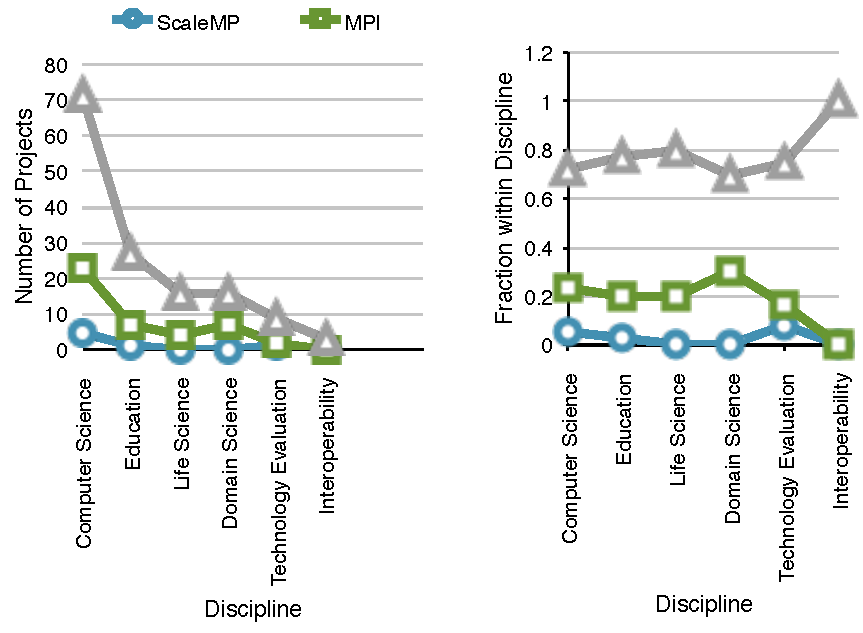
\includegraphics[width=1.0\textwidth]{images/trend-b.pdf}
  \caption{Requests by of technologies by discipline within a
    project. $\bigtriangleup$ = Map Reduce, Hadoop, or Twister,
    $\Box$\footnote{slash box does not show up, do we need another
      latex package}
  = MPI, $\circ$ = ScaleMP}
\end{figure}



\begin{figure}[htb]
  \centering
    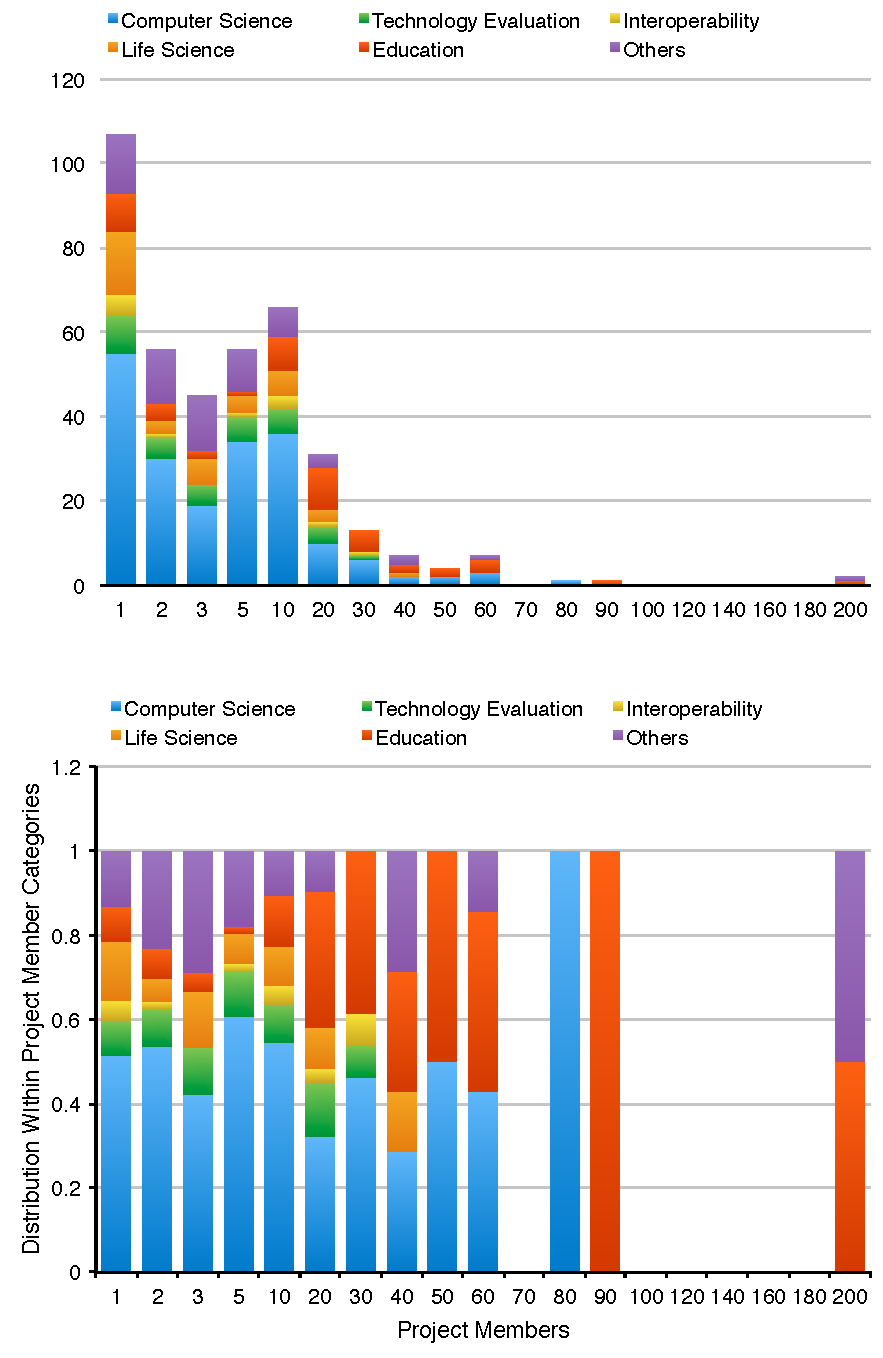
\includegraphics[width=1.0\textwidth]{images/project-member-dist.pdf}
  \caption{Project Member Dist.}
\end{figure}

\afterpage{\clearpage}

\FILE{devops.tex}

\section{System Management}

The goals of FutureGrid to offer a variety of services as part of its
testbed features is going beyond services that are normally offered by
data and supercomputing centers for research. This provides a number
of challenges that need to be overcome in order to efficiently manage
the system and provide services that have never been offered to users
as they exist on FutureGrid.

\subsection{Integration of Systems and Development Team}

FutureGrid started initially with a model where the systems team and
the software team were separated. A clear wall of responsibilities was
erected that resulted in multiple challenges:

\begin{enumerate}

\item
The system setup and management was completely separated from
the software development team focussing mostly on the deployment of
existing technologies. 

\item
The system was complex, but its deployment was documented to a limited
extend not allowing the developers to utilize it properly.

\item 
Lack of trust by the systems team dis not allow the software team to
have a valid development environment.

\item
The software developed needed a testbed within the
testbed that was not necessarily reflecting the actual system setup.

\end{enumerate}

Together these issues, made it extremely difficult if not impossible to
further any development in regards to the design of a testbed
infrastructure as requested by our original ambitious goals. 

To overcome these difficulties it was decided that the systems team
must be integrated in some fashion into the software team and become
part of the development process. This integration is not an isolated
instance within FutureGrid, but is also executed in many modern data
centers and is now recognized with its own term called {\em DevOps}.

\subsection{DevOps}

Devops is not just a buzzword from industry and research communities,
but it provides value added processes to the deployment and
development cycles that are part of modern data centers. It can today
be understood as a software development method that stresses
collaboration and integration between software developers and
information technology professionals such as a system administrator. 

WHile using an infrasrtructure such as clouds we recognized early on
that the lifetime of a particular IaaS framework is about 3-6 month
before a new version is installed. This is a significant difference to
a traditional High Performance Computing Center that is comprised of
many software tools experiencing much longer life spans. This is not
only based on security patches but significant changes for example in
the evolving security, user services as well as the deployment of new
services that become avalable in rapid procession.

This rapid change of the complex infrastructure requires a rethinking
about how systems in general are menaged and how they can be made
avalable to the development teams. While previously it may have been
enough to install updates on the machines, DevOps frameworks provide
the developer and system administarors to create and share
enviroenments that are used in production and development while at the
same time increasing quality assurance by leveraging each others
experiences (see Figure \ref{F:devops}).

\begin{figure}[htb]
  \centering
   \begin{minipage}{.5\textwidth}
    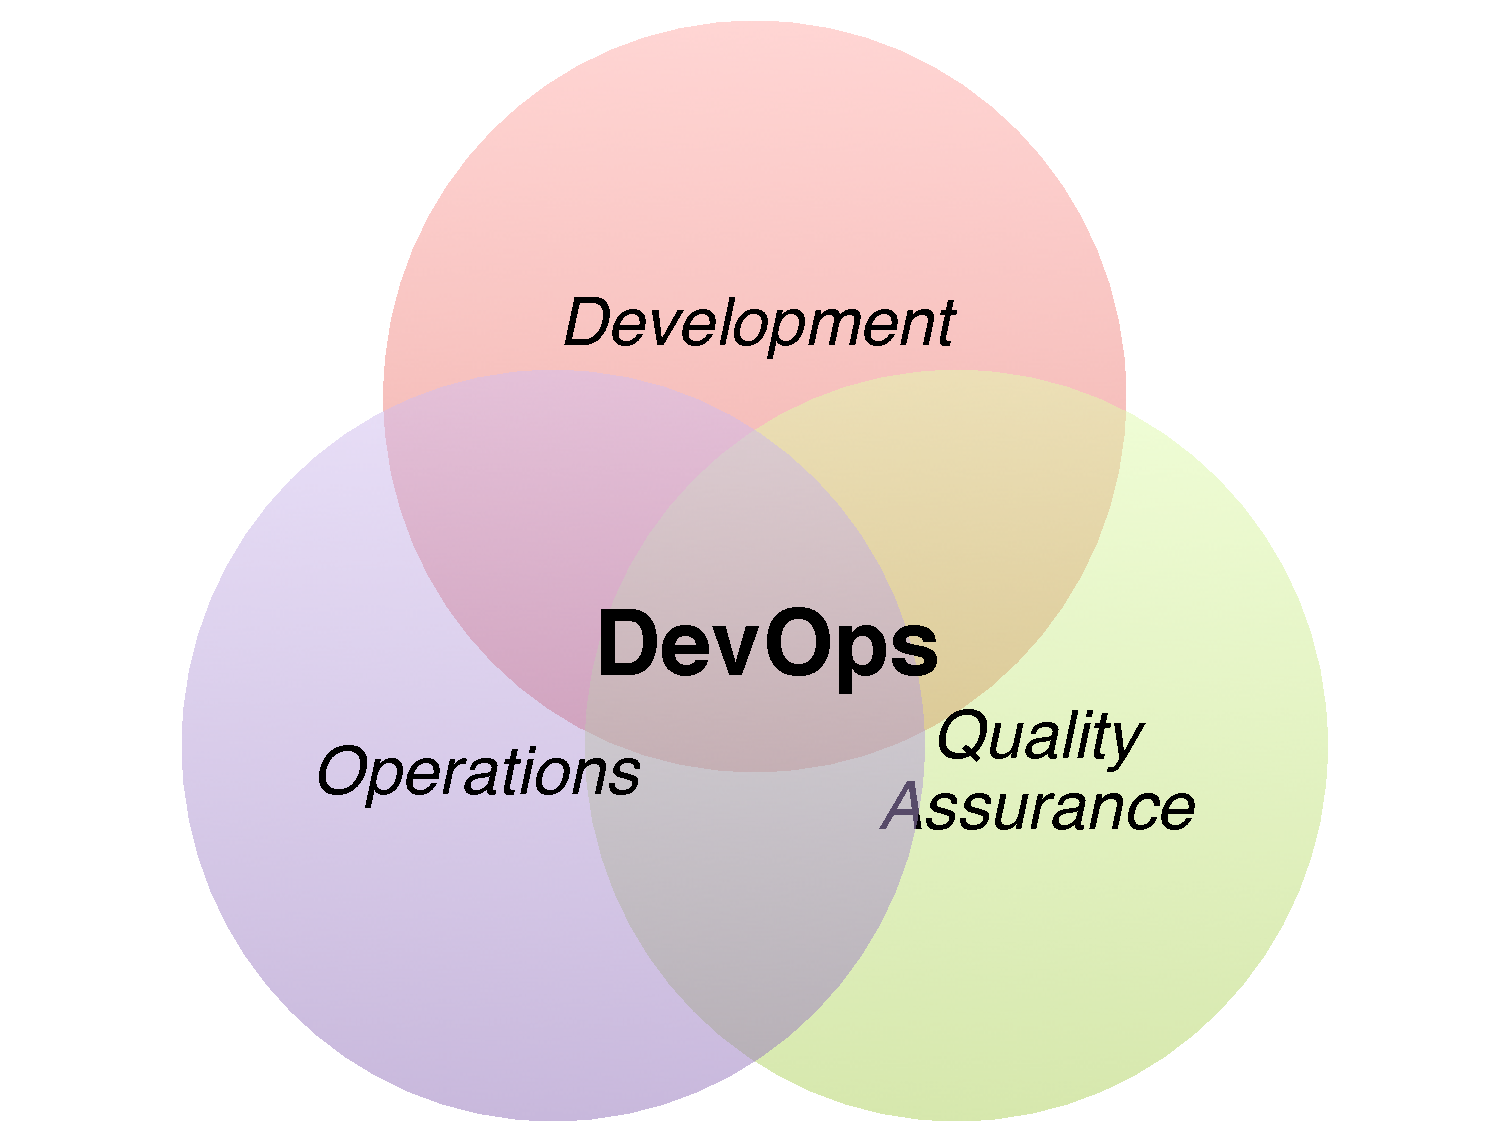
\includegraphics[width=1.0\textwidth]{images/devops.pdf}
    \caption{DevOps Intersection.}
    \label{F:devops}
  \end{minipage}%
   \begin{minipage}{.5\textwidth}
     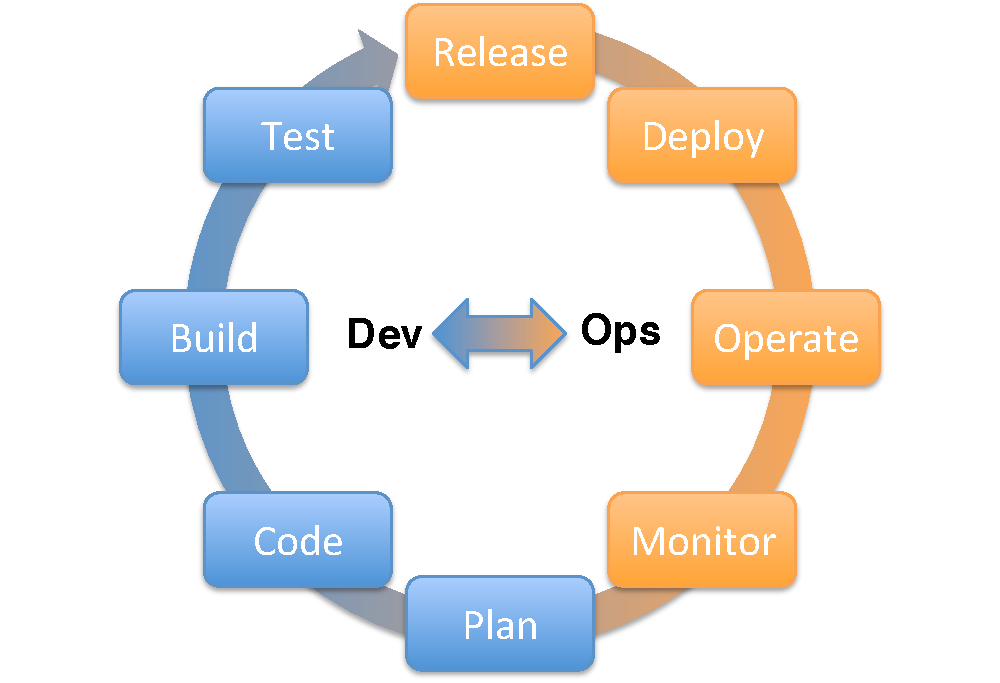
\includegraphics[width=1.0\textwidth]{images/devops-circle.pdf}
     \caption{DevOps Cycle.}
     \label{F:devops-circel}
  \end{minipage}%
\end{figure}

\subsection{DevOps Cycle}

While combining the steps executed by the Development and operational
team from planing, to coding, building and testing, to the release,
deployment and operation and monitoring (see Figure
\ref{F:devops-circle}), each of the phases provides a direct feedback
between the DevOps team members and shortening thus the entire
development phase. It also allows to test out new services and
technologies in a rapid progression. Hence it is possible to roll out
new developments much faster into production. This leads to a much mor
rapid integrated cycle than without the correlation between
development and operation would be possible.

\subsection{DevOps Supporting Tools}

A number of tools are available that make the introduction of DevOps
strategies more efficient. The first is the need for an efficient
communication pathway to manage tasks not only between developers but
also between users. Thus the ideal system would provide a complete
integration of a project management system that allows to manage tasks
for both developers and operators, but also to easily integrate
tickets and transform them into tasks. In XSEDE and other
supercomputing centers a system called RT is typically used for user
ticket management. Other systems such as jira, mantis, and ??? are
often used to manage the software and systems related
tasks. Unfortunately, personal or organizational constraints prevent
often the integration of the two systems and additional overhead is
needed to move user tickets into tasks and the development
cycle. Within FutureGrid we experimented as part of our opensource
development extensively with jira as systems and ticketing system
reveling that newest development in such areas motivated by DevOps
teams lead to tools that support the overall cycle including users
(see Figure \ref{F:usedevops}). However, the integration of
FutureGrid within the overall much larger XSEDE effort did make it not
possible to switch from RT to jira for user ticket
management. To stress this user integration we term this framework
{\em UseDevOps}. Tools to integrate Development and Operation
deployment include puppet, chef, ansible, cfengine and bcfg2. While
FutureGrid started out with bcfg2 we have since than switched to other
tools due to their prevalence within the community. Chef, puppet, and
ansible have significant amount of traction. Due to expertise within
our group we currently explore chef and ansible. 

\begin{figure}[htb]
  \centering
    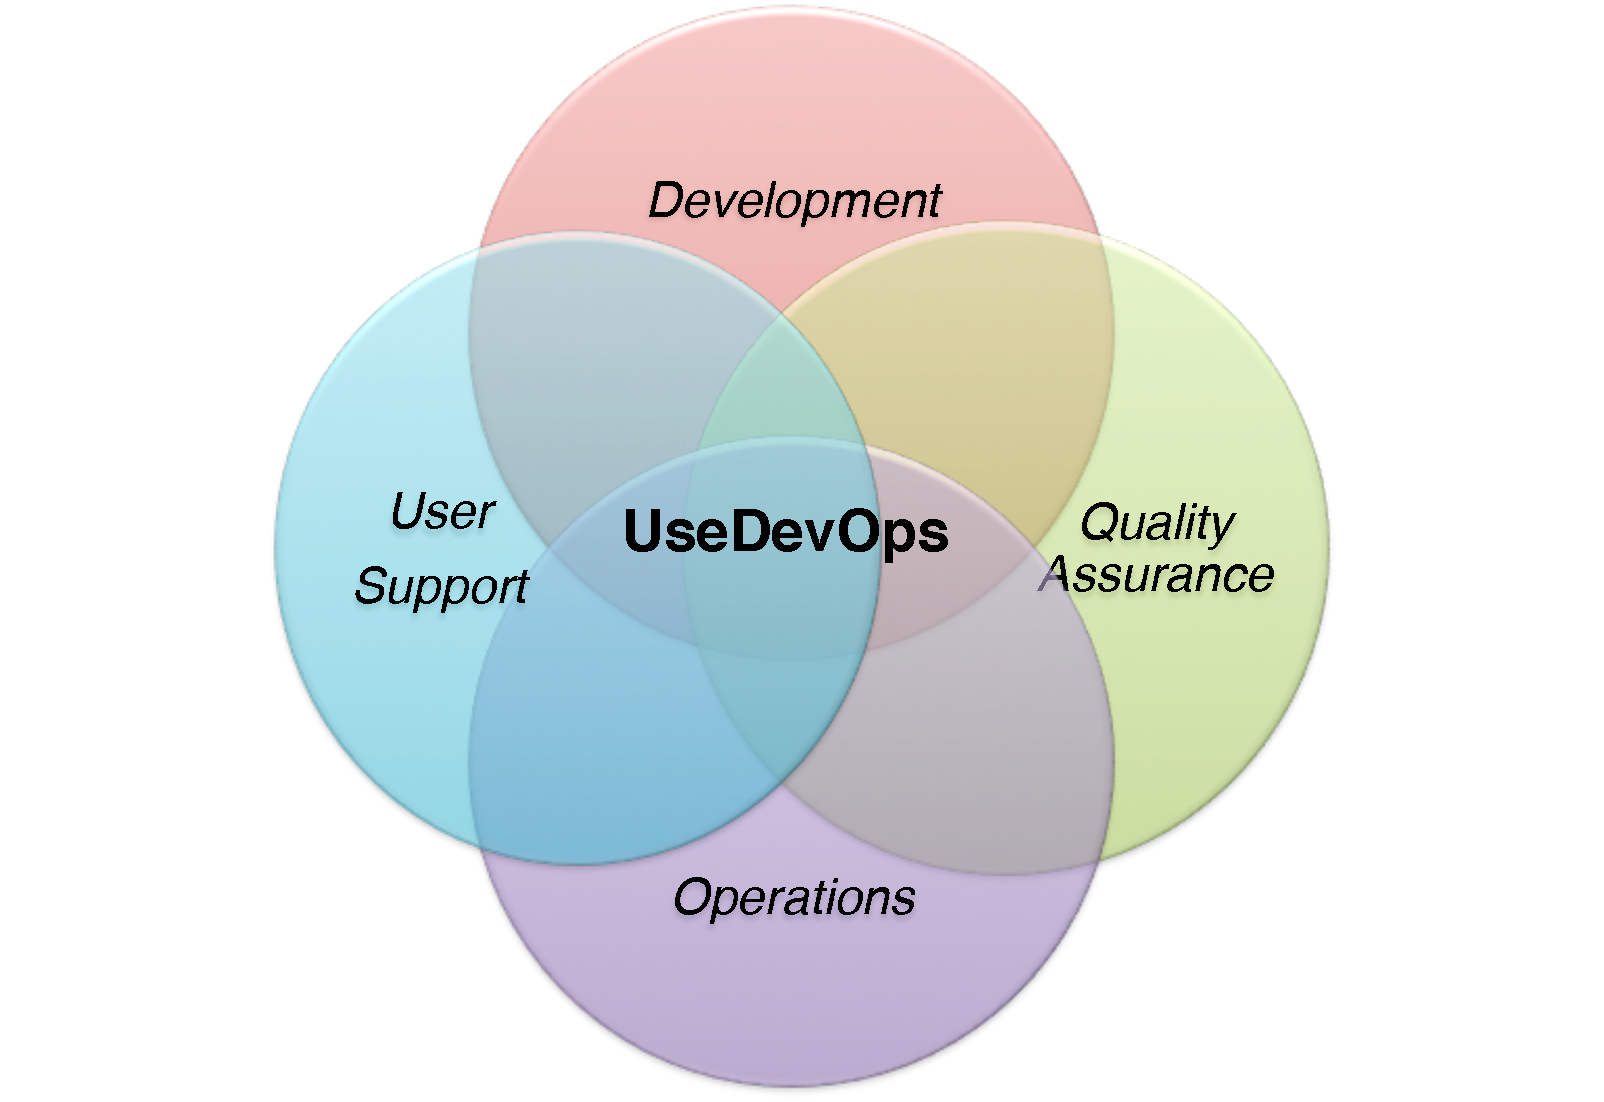
\includegraphics[width=0.5\textwidth]{images/usedevops.pdf}
  \caption{User Support integrated into DevOps leads to UseDevops.}
  \label{F:usedevops}
\end{figure}








%http://en.wikipedia.org/wiki/DevOps








\subsection{Support for Educational Services}

manual

reprovisioning

reconfiguration




\FILE{cloudmesh.tex}

\section{Cloudmesh\footnote{This section is als available in part from
  the cloudmesh Web pages and includes large protions of copied
  text. The text is publically available.}}\label{S:cloudmesh}

From the experience with FutureGrid we identified the need for a more
tightly integrated software infrastructure addressing the need to
deliver a software-defined system – encompassing virtualized and
bare-metal infrastructure, networks, application, systems and platform
software – with a unifying goal of providing Cloud Testbeds as a
Service (CTaaS). This system is termed cloudmesh to symbolize (a) the
creation of a tightly integrated mesh of services targeting multiple
IaaS farmeworks (b) the ability to federate a number of resources from
from academia and industry. This includes existing FutureGrid
infrastructure, Amazon Web Services, Azure, HP Cloud, Karlsruhe using
not only one IaaS framework but various. (c) The creation of an
environment in which it becomes more easy to experiment with platforms
and softwere services while assiting to deploy them more easily.
In addition to virtual resources, FutureGrid exposes bare-metal
provisioning to users, but also a subset of HPC monitoring
infrastructure tools. Services will be available through command line,
API, and Web interfaces.

\subsection{Functionality}

Cloudmesh provides due to its integrated services the ability to be an
onramp for other clouds. It also provides information services to
various system level sensors to give access to sensor and utilization
data. They internally can be used to optimize the system
usage. The provisioning experience from FutureGrid has taught us that
we need to provide the creation of new clouds, the repartitioning of
resources between services (cloud shifting), and the integration of
external cloud resources in case of over provisioning (cloud
bursting). As we deal with many IaaS we need an abstraction layer on
top of the IaaS framework. Experiment management is conducted with
workflows controoled in shells, Python/iPython, as well as systems
such as Heat, Accounting is supported through additional services such
as user management and charge rate management. Not all features are
yet implemented. Figure \label{F:cm-func} shows the main functionality
that we target at this time to implement.

\begin{figure}[h!]
  \centering
    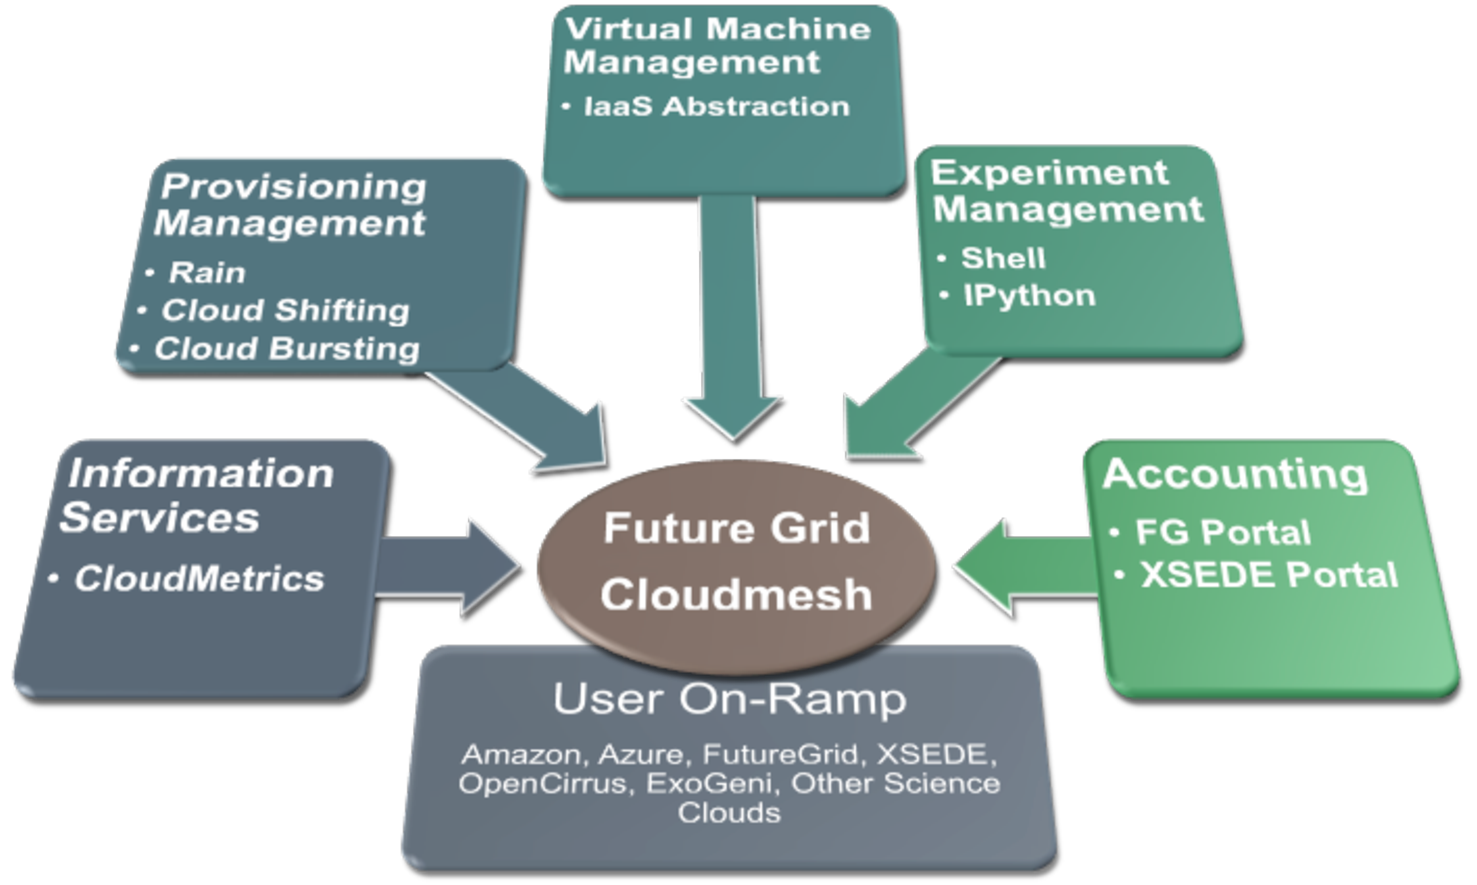
\includegraphics[width=1.0\textwidth]{images/cm-functionality.pdf}
  \caption{CM Functionality.}\label{F:cm-func}
\end{figure}


\subsection{Architecture}

The three layers of the Cloudmesh architecture include a Cloudmesh
Management Framework for monitoring and operations, user and project
management, experiment planning and deployment of services needed by
an experiment, provisioning and execution environments to be deployed
on resources to (or interfaced with) enable experiment management, and
resources.

\begin{figure}[h!]
  \centering
    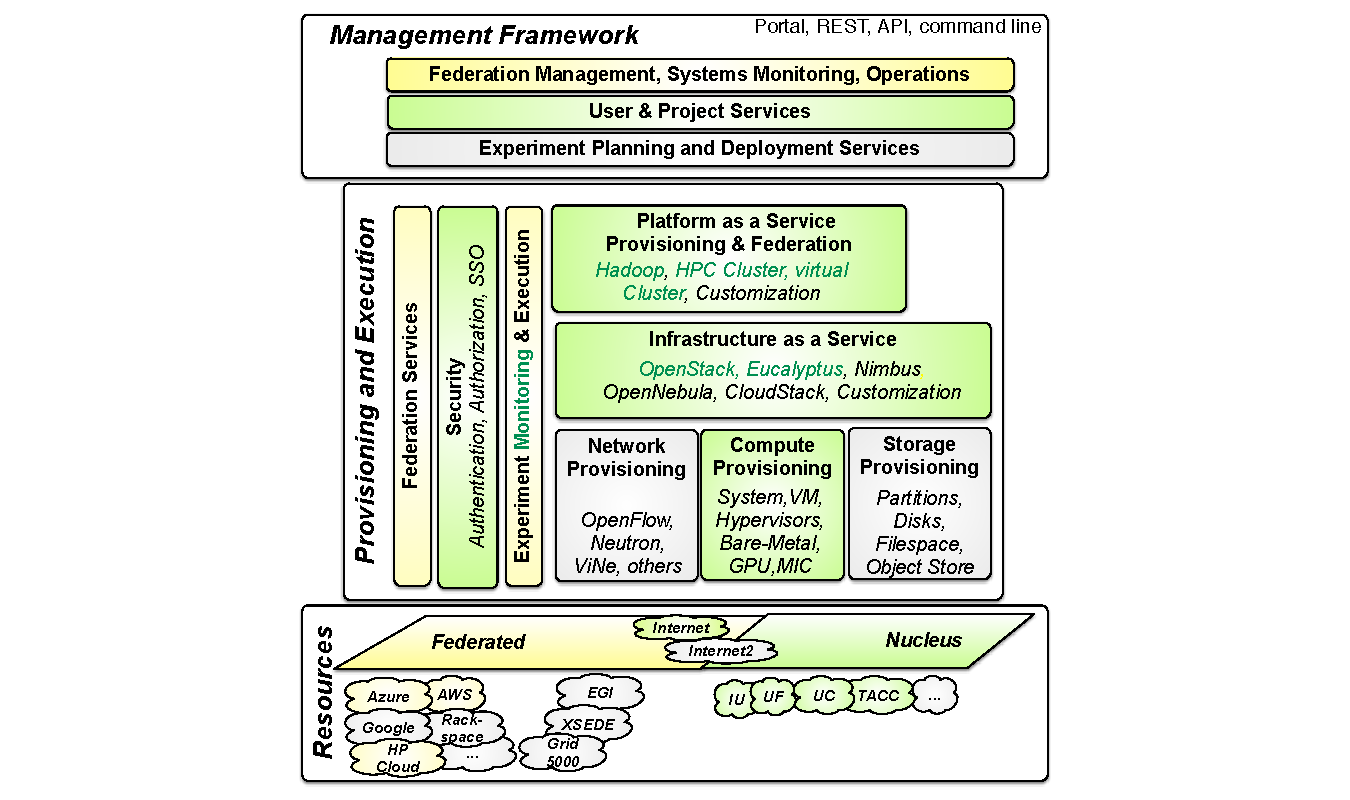
\includegraphics[width=1.0\textwidth]{images/cm-arch.pdf}
  \caption{CM Architecture.}
\end{figure}

\paragraph{System Monitoring and Operations.}

The management framework contains services to facilitate FutureGrid day-to-day operation, including federated or selective monitoring of the infrastructure. Cloudmesh leverages FutureGrid for the operational services and allows administrators to view ongoing system status and experiments, as well as interact with users through ticket systems and messaging queues to inform subscribed users on the status of the system.
The cloudmesh management framework offers services that simplify integration of resources in the FutureGrid nucleus or through federation. This includes, for user management, access to predefined setup templates for services in enabling resource and service provisioning as well as experiment execution. To integrate IaaS frameworks cloudmesh offers two distinct services:

(a) a federated IaaS frameworks hosted on FutureGrid,
(b) the availability of a service that is hosted on FutureGrid allowing the “integration” of IaaS frameworks through user credentials either registered by the users or automatically obtained from our distributed user directory.

For (b) several toolkits exist to create user-based federations, including our own abstraction level which supports interoperability via libcloud, but more importantly it supports directly the native OpenStack protocol and overcomes limitations of the EC2 protocol and the libcloud compatibility layer. Plugins that we currently develop will enable access to clouds via firewall penetration, abstraction layers for clouds with few public IP addresses and integration with new services such as OpenStack Heat. We successfully federated resources from Azure, AWS, the HP cloud, Karlsruhe Institute of Technology Cloud, and four FutureGrid clouds using various versions of OpenStack and Eucalyptus. The same will be done for OpenCirrus resources at GT and CMU through firewalls or proxy servers.
Additional management flexibility will be introduced through automatic cloud-bursting and shifting services. While cloud bursting will locate empty resources in other clouds, cloud shifting will identify unused services and resources, shut them down and provision them with services that are requested by the users. We have demonstrated this concept in 2012, moving resources for ~100 users to services that were needed based on class schedules. A reservation system will be used to allow for reserved creation of such environments, along with improvements of automation of cloud-shifting.

\paragraph{User and Project Services}

FutureGrid user and project services simplify the application processes needed to obtain user accounts and projects. We have demonstrated in FutureGrid the ability to create accounts in a very short time, including vetting projects and users – allowing fast turn-around times for the majority of FutureGrid projects with an initial startup allocation. Cloudmesh re-uses this infrastructure and also allows users to manage proxy accounts to federate to other IaaS services to provide an easy interface to integrate them.

\paragraph{Accounting and App Store}

To lower the barrier of entry Cloudmesh will be providing a shopping cart which will allow checking out of predefined repeatable experiment templates. A cost is associated with an experiment making it possible to engage in careful planning and to save time by reusing previous experiments. Additionally, the Cloudmesh App Store may function as a clearing-house of images, image templates, services offered and provisioning templates. Users may package complex deployment descriptions in an easy parameter/form-based interface and other users may be able to replicate the specified setup with.
Due to our advanced Cloudmesh Metrics framework we are in the position to further develop an integrated accounting framework allowing a usage cost model for users and management to identify the real impact of an experiment on resources. This will be useful to avoid overprovisioning and inefficient resource usage. The cost model will be based not only on number of core hours used, but also the capabilities of the resource, the time, and special support it takes to set up the experiment. We will expand upon the metrics framework of FutureGrid that allows measuring of VM and HPC usage and associate this with cost models. Benchmarks will be used to normalize the charge models.

\paragraph{Networking.}

We have a broad vision of resource integration in FutureGrid with systems offering different levels of control from “bare metal” to use of a portion of a resource. Likewise, we must utilize networks offering various levels of control, from standard IP connectivity to completely configurable SDNs as novel cloud architectures will almost certainly leverage NaaS and SDN alongside system software and middleware. FutureGrid resources will make use of SDN using OpenFlow whenever possible and the same level of networking control will not be available in every location.

\paragraph{Monitoring.}

To serve the purposes of CISE researchers, Cloudmesh must be able to access empirical data about the properties and performance of the underlying infrastructure beyond what is available from commercial cloud environments. To accommodate this requirement we have developed a uniform access interface to virtual machine monitoring information available for OpenStack, Eucalyptus, and Nimbus. In the future, we will be enhancing the access to historical user information. Right now they are exposed through predefined reports that we create on a regular basis. To achieve this we will also leverage the ongoing work while using the AMPQ protocol. Furthermore, Cloudmesh will provide access to common monitoring infrastructure as provided by Ganglia, Nagios, Inca, perfSonar, PAPI and others.

\begin{figure}[h!]
  \centering
    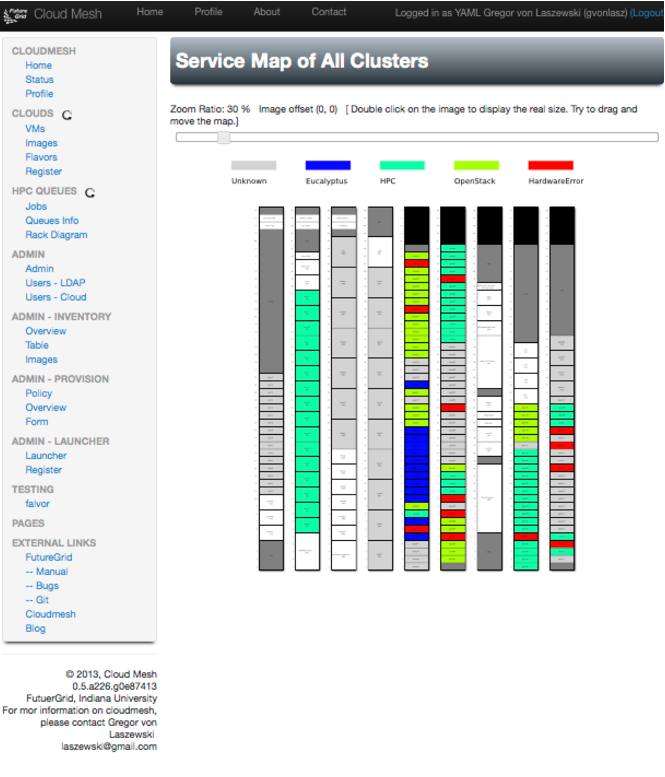
\includegraphics[width=.7\textwidth]{images/rainbow.pdf}
  \caption{Monitoring the Service distribution of FutureGrid with cloudmesh.}
\end{figure}

\subsection{Cloud Shifting}

We have already demonstrated via the RAIN tool in cloudmesh that it is
possible to easily shift resources between services. We are currently
expanding upon this idea and developing more easy to use user
interfaces that assit administrators and users through role and
project based authentication to move resources from one service to
another (see Figure \ref{F:shift}).

\begin{figure}[h!]
  \centering
    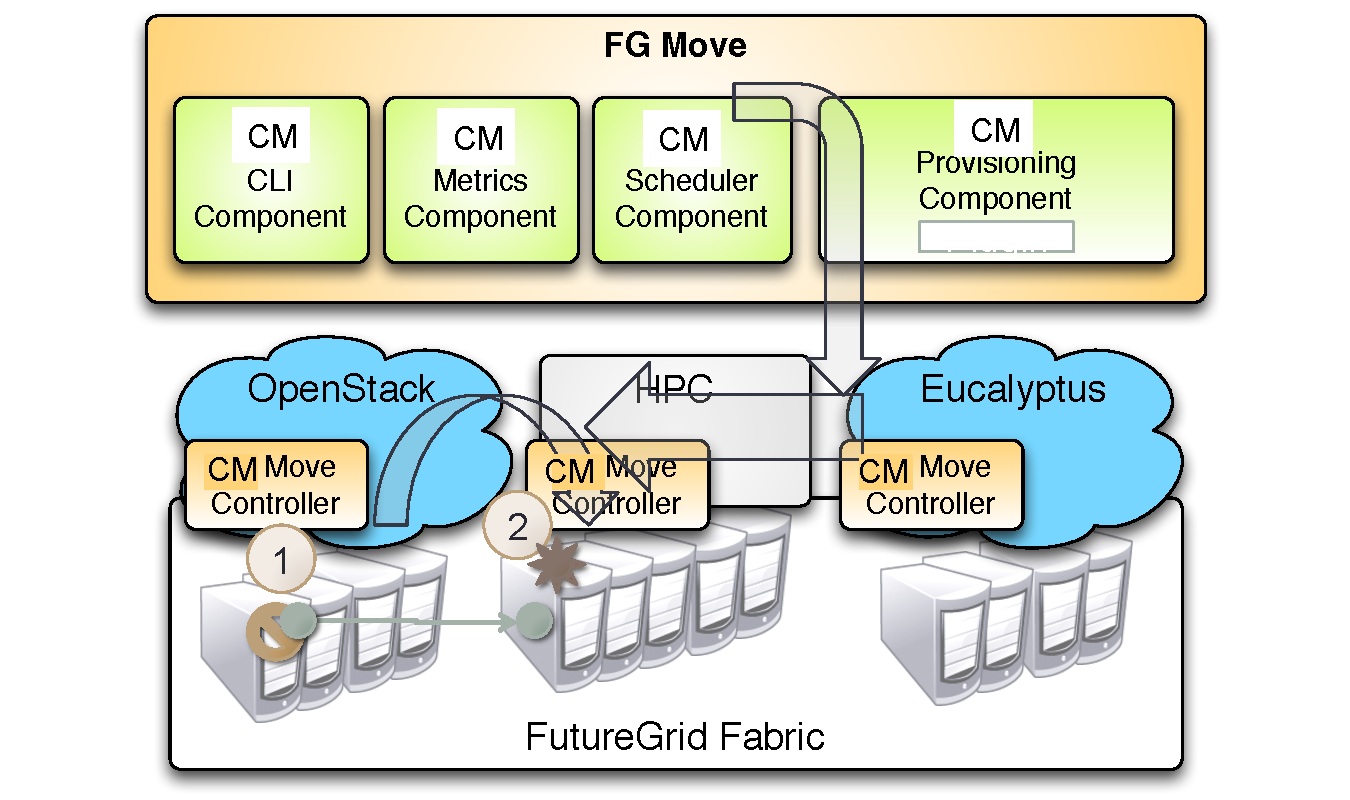
\includegraphics[width=1.0\textwidth]{images/shift2.pdf}
  \caption{Shifting resources makes it possible to offer flexibility
    in the service distribution in case of over or underprovisioning.}\label{F:shift}
\end{figure}

\subsection{Graphical User Interface}

Despite the fact that cloudmesh was originally a quite sophisticated
command shell and commandline tool, we have spend recently more time
in exposing this functionality through a conveneient Web
interface. Some mor popular views if this interface are depicted in
Figure \ref{F:instances} hinting on how easy it is with a single
button to create multiple VMs accross a variety of IaaS. Also nice is
that this not only includes resources at IU but also at external
locations. Pushing this easy management in a more sophisticated
experience for the user while associating one-click deployments that
include the ability to deploy virtual clusters, hadoop environments,
and other more elaborate setups wie provide an early prototype
screenshot in Figure \ref{F:oneclick}.

\begin{figure}[htb]
  \centering
    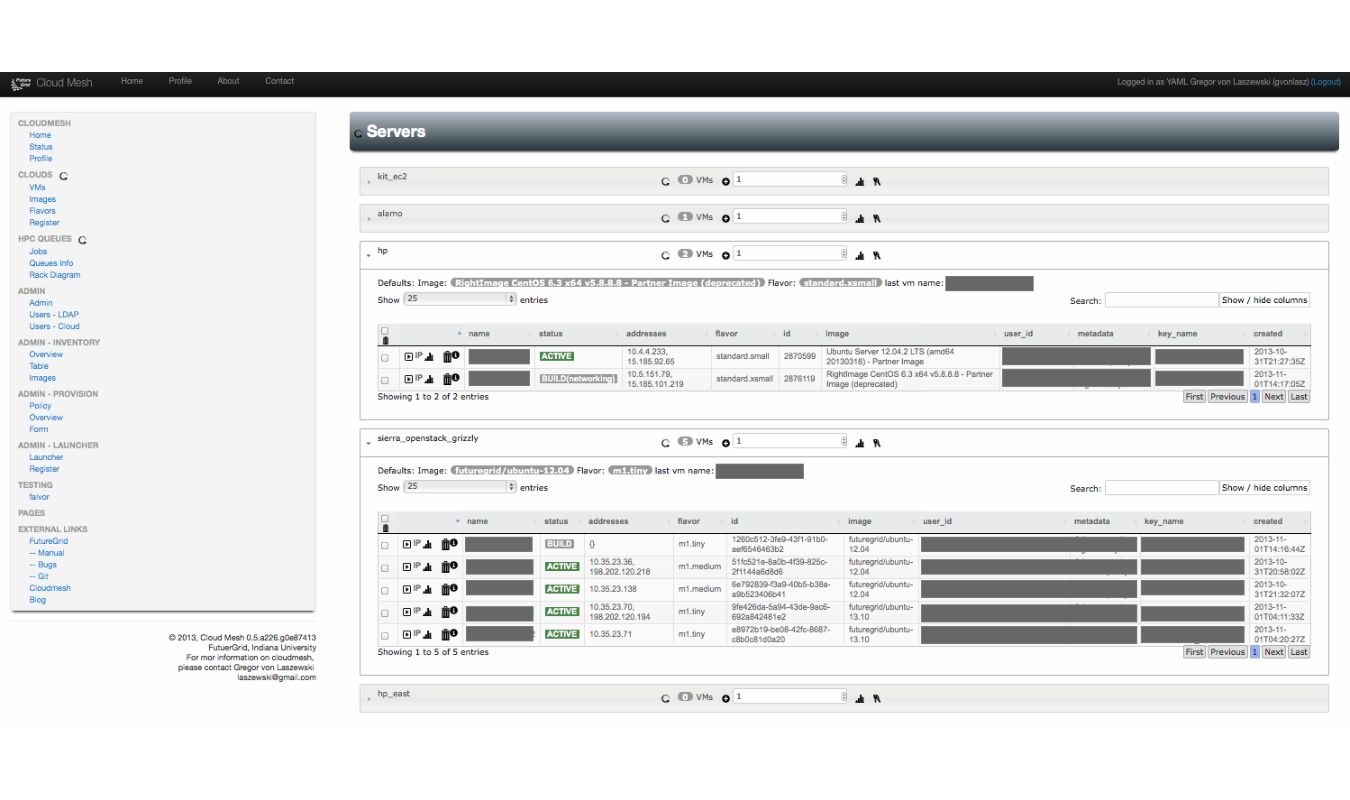
\includegraphics[width=.9\textwidth]{images/instances.pdf}
  \caption{Rainbow.}\label{F:instances}
  \centering
    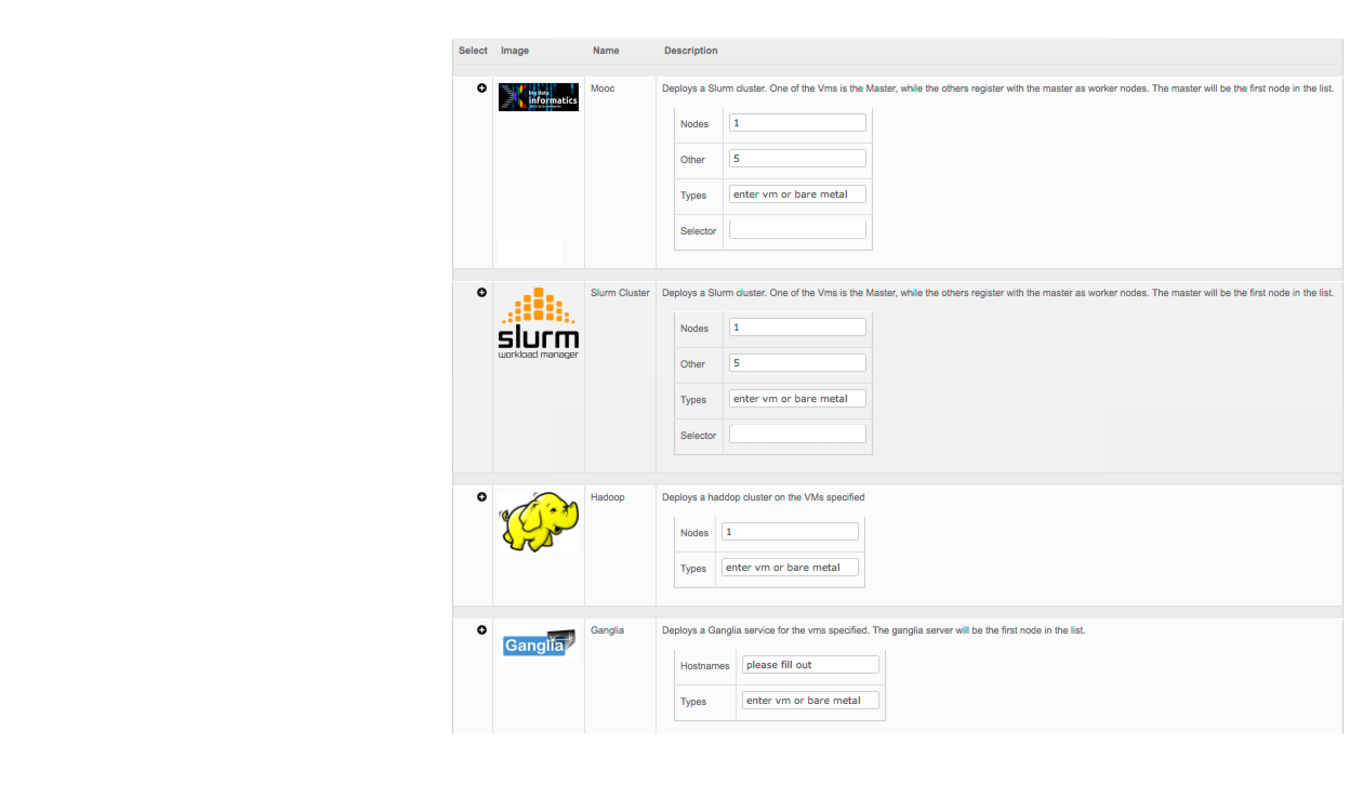
\includegraphics[width=.9\textwidth]{images/oneclick.pdf}
  \caption{One click deployment of platforms and sophisticated
    services that could even spawn multiple resources.}\label{F:oneclick}
\end{figure}


\afterpage{\clearpage}



\section*{Acknowledgement}

Some of the text published in this chapter is available form the
FutureGrid portal. The FutureGrid project is funded by the National
Science Foundation (NSF) and is led by Indiana University with
University of Chicago, University of Florida, San Diego Supercomputing
Center, Texas Advanced Computing Center, University of Virginia,
University of Tennessee, University of Southern California, Dresden,
Purdue University, and Grid 5000 as partner sites. This material is
based upon work supported in part by the National Science Foundation
under Grant No. 0910812. If you use FutureGrid and produce a paper or
presentation, we ask you to include the reference
\cite{las2010gce,las12fg-bookchapter}.

\bibliographystyle{IEEEtranS}
\bibliography{%
bib/references,%
bib/vonLaszewski-jabref,%
bib/image-refs,%
bib/cyberaide-cloud,%
bib/python}

%%%%%%%%%%%%%%%%%%%%%%%%%%%%%%%%%%%%%%%%%%%%%%%%%%%%%%%%%%%%
\clearpage

\appendix

\FILE{overview.tex}

\section{Overview}

FutureGrid is a national-scale Grid, Cloud and HPC computing test-bed service of modest size that includes a number of computational resources at five distributed locations. FutureGrid experience and architecture is built around software defined systems at all levels of the stack shown in figure – encompassing VM and bare-metal infrastructure, networks and application, systems and platform software – with a unifying goal of providing Computing Testbeds as a Service. FutureGrid systems total 4704 cores divided into distributed general purpose clusters at Chicago, Florida, IU and TACC; a Cray XT5m at IU and four small specialized clusters supporting SSD (at SDSC), Large Disk Large memory (at IU) and NVIDIA GPU’s (IU). FutureGrid’s system model has grown in sophistication and now supports software-defined systems – encompassing virtualized and bare-metal infrastructure, networks, application, systems and platform software – with a unifying goal of providing Cloud Testbeds as a Service (CTaaS). Cloudmesh aggregates resources not only from FutureGrid, but also from OpenCirrus, Amazon, Microsoft Azure, and HP Cloud and GENI resources. Cloudmesh was originally developed in order to simplify the execution of multiple concurrent experiments on a federated cloud infrastructure and in addition to virtual resources, FutureGrid exposes bare-metal provisioning to users.

Users can apply for projects either at FutureGrid or XSEDE portals. A single account provides a user access to all FutureGrid machines and we can describe the type of work that can be done by looking at FutureGrid’s experience based on 3 and a half years of operation with 355 projects and 2178 users from 55 countries with 76\% from the USA. 51.8\% of these projects were mainly computer science (including middleware and cyberinfrastructures) research, 9.6\% technology evaluation, 13.2\% education, 9.6\% in life sciences and 11.5\% in other application domains. We looked in detail at the last 200 projects starting October 25 2011 to understand in more detail usage paradigms. 98 of these projects needed only virtual machine (VM) access and 54 requested both virtualized and non-virtualized nodes. Of the 48 projects not requesting VM’s, 8 were studying cloud technology like Hadoop and so 160 projects (80\%) were cloud related. 16 projects involved GPU access and 30\% of all projects used MapReduce in some way. The use of FutureGrid for education has been increasing and 21\% of projects in last 2 years have been for education dividing into 29 semester length classes and the 13 remaining split between REU training, Summer Schools, Tutorials, and workshops. Of 42 education requests, 36 were computer science, 3 application oriented and 3 mixed. These education classes covered areas like cloud computing, distributed systems, parallel computing, big data, data-intensive computing and datamining, business analytics, autonomic computing, cyberinfrastructure, storage, software carpentry, data centers and large scale infrastructure, MapReduce, high performance computing, networking, science clouds, and particular tools supported on FutureGrid.
Coming to the 136 research projects, 109 had a major CS component and 44 an application component with 17 of these jointly classified. Application projects included 18 from bioinformatics including genomics, radiology, cardiovascular simulation, surgery control, health sensors, iPlant cyberinfrastructure and text mining. Only 10 application projects had a simulation (major focus of most HPC systems) focus including combustion, CFD, subsurface modeling, climate, weather, ocean, environment, earthquakes and supply chains. Physical science and engineering data intensive applications (8 projects) include astronomy, particle physics, aerospace reliability, ocean observation, hydroinformatics, GIS and accelerator control. 6 social science projects include conflict resolution, disaster management using Twitter, optimization, political science and economics.

Turning to CS related projects, 23 were in basic virtualization (IaaS) areas. They included provisioning, deployment, new hypervisors including increased performance, elasticity and scheduling, resource management, benchmarking, emulation, and IaaS scaling to support MOOC’s. 4 projects studied distributed clouds and storage with federation. 3 projects centered on networking (routing, optimized devices and emulation) and 2 studied software engineering for clouds. 5 projects were aimed at cyberphysical systems with health, power and mobile applications and FutureGrid used for control and support analytics. 2 projects had a P2P focus covering security and fault tolerance. Security was popular with 10 projects covering trusted P2P storage, mobile and other clients, intrusion detection, file sharing, confidentiality and integrity of data, vulnerability, watermarks and hybrid clouds with different security models. There were 4 HPC programming language projects and 8 covering cloud programming with scheduling, fault tolerance and runtime. 5 fault tolerance projects covered P2P, MapReduce, workflow and HPC. 4 projects covered distributed software transactional memory and concurrency control. Data systems were very popular with 13 projects covering cloud storage, data transfer, NoSQL, streaming big data, Apache software stack, analytics, image retrieval, testing, provenance and the semantic web. 2 projects studied enterprise software issues. 9 artificial intelligence projects covered learning networks for images and social media, large scale image classification by clustering, machine learning, text mining, and agents. Network science with 3 projects saw use of NoSQL datastores to study Twitter, a major infrastructure to support graph and other tools and community detection. Finally 13 projects focused on cyberinfrastructure middleware with XSEDE and EMI (European Middleware initiative) systems, software as a service for HPC simulations, HPC clouds, MPI porting, fault tolerance, workflow, scheduling and resource management, tools, logging and performance.
There were 19 Evaluation projects which covered XSEDE testing (a major actual and intended use of FutureGrid), Open Science Grid testing, particle physics, Apache Big Data stack, Solid State disks, comparison of different VM frameworks, familiarization with cloud technology, GPU’s and studies aimed at planning institutional initiatives in cloud computing. There were 3 Interoperability projects involving long term support of standard end-points. 

FutureGrid interacts with XSEDE on integrating accounting approaches, EOT and software testing.


\end{document}
